\documentclass[../main.tex]{subfiles}

\begin{document}

\label{cha:cha_P_14_3_3}
\subsection{Quantification of Error of Linear Regression}

\noindent Any line other than the one computed in Example 14.4 results in a larger sum of the squares of the residuals. Thus, the line is unique and in terms of our chosen criterion is a ``best'' line through the points. A number of additional properties of this fit can be elucidated by examining more closely the way in which residuals were computed. Recall that the sum of the squares is defined as [Eq. (14.12)]

\begin{equation}
	\tag{14.17}
	S_r = \sum^n_{i=1} (y_i - a_0 - a_1 x_i)^2
\end{equation}

Notice the similarity between this equation and Eq. (14.4)

\begin{equation}
\tag{14.18}
S_t = \sum (y_i - \bar{y})^2
\end{equation}
In Eq. (14.18), the square of the residual represented the square of the discrepancy between the data and a single estimate of the measure of central tendency-the mean. In Eq. (14.17), the square of the residual represents the square of the vertical distance between the data and another measure of central tendency-the straight line (\ref{fig:fig_14_9}).

\begin{wrapfigure}{l}{0.25\textwidth}
    \centering
    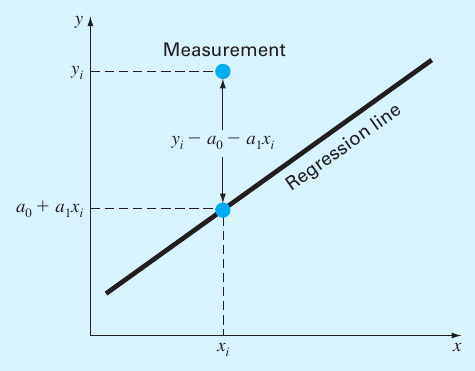
\includegraphics[width=0.25\textwidth]{fig_14_9}
   \caption{\textsf{The residual in linear regression represents the vertical distance between a data point and the straight line.}}
   \label{fig:fig_14_9}
\end{wrapfigure}

The analogy can be extended further for cases where (1) the spread of the points around the line is of similar magnitude along the entire range of the data and (2) the distribution of these points about the line is normal. It can be demonstrated that if these criteria are met, least-squares regression will provide the best (i.e., the most likely) estimates of $a_0$ and $a_1$ (Draper and Smith, 1981). This is called the maximum likelihood principle in statistics. In addition, if these criteria are met, a ``standard deviation'' for the regression line can be determined as [compare with Eq. (14.3)]

\begin{equation}
	\tag{14.19}
	s_{y/x} = \sqrt{\frac{S_r}{n-2}}
\end{equation}

\noindent where $s_{y/x}$ is called the \textit{standard error of the estimate}. The subscript notation ``$y/x$'' designates that the error is for a predicted value of $y$ corresponding to a particular value of $x$.
Also, notice that we now divide by $n - 2$ because two data-derived estimates - $a_0$ and $a_1$ - were used to compute $S_r$; thus, we have lost two degrees of freedom. As with our discussion of the standard deviation, another justification for dividing by $n - 2$ is that there is no such thing as the ``spread of data'' around a straight line connecting two points. Thus, for the case where $n = 2$, Eq. (14.19) yields a meaningless result of infinity.

Just as was the case with the standard deviation, the standard error of the estimate quantifies the spread of the data. However, $s_{y/x}$ quantifies the spread \textit{around the regression line} as shown in \ref{fig:fig_14_10b} in contrast to the standard deviation $s_y$ that quantified the \textit{spread around the mean} (\ref{fig:fig_14_10a}).

\begin{figure}[H]
	\centering
	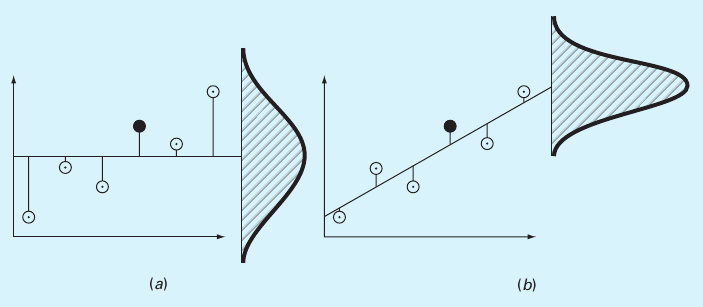
\includegraphics[width=1\linewidth]{fig_14_10}
	\caption{\textsf{Regression data showing (a) the spread of the data around the mean of the dependent variable and (b) the spread of the data around the best-fit line. The reduction in the spread in going from (a) to (b), as indicated by the bell-shaped curves at the right, represents the improvement due to linear regression.}}
	\label{fig:fig_14_10}
	\label{fig:fig_14_10a}
	\label{fig:fig_14_10b}
\end{figure}

\begin{figure}[H]
	\centering
	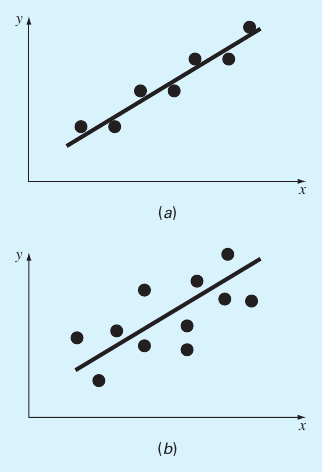
\includegraphics[width=1\linewidth]{fig_14_11}
	\caption{\textsf{Examples of linear regression with (a) small and (b) large residual errors.}}
	\label{fig:fig_14_11}
	\label{fig:fig_14_11a}
	\label{fig:fig_14_11b}
\end{figure}

These concepts can be used to quantify the ``goodness'' of our fit. This is particularly useful for comparison of several regressions (\ref{fig:fig_14_11a}). To do this, we return to the original data and determine the total sum of the squares around the mean for the dependent variable (in our case, $y$). As was the case for Eq. (14.18), this quantity is designated $S_t$. This is the magnitude of the residual error associated with the dependent variable prior to regression. After performing the regression, we can compute $S_r$, the sum of the squares of the residuals around the regression line with Eq. (14.17). This characterizes the residual error that remains after the regression. It is, therefore, sometimes called the unexplained sum of the squares. The difference between the two quantities, $S_t - S_r$, quantifies the improvement or error reduction due to describing the data in terms of a straight line rather than as an average value. Because the magnitude of this quantity is scale-dependent, the difference is normalized to $S_t$ to yield

\begin{equation}
	\tag{14.20}
	r^2 = \frac{S_t - S_r}{S_t}
\end{equation}

\noindent where $r^2$ is called the \textit{coefficient of determination} and $r$ is the \textit{correlation coefficient} ($=\sqrt{r^2}$). For a perfect fit, $S_r = 0$ and $r^2 = 1$, signifying that the line explains 100\% of the variability of the data. For $r^2 = 0$, $S_r = S_t$ and the fit represents no improvement. An alternative formulation for $r$ that is more convenient for computer implementation is

\begin{equation}
	\tag{14.21}
	r = \frac{n \sum (x_i y_i) - (\sum x_i) (\sum y_i)}{\sqrt{n \sum x^2_i - (\sum x_i)^2} \sqrt{n \sum y^2_i - (\sum y_i)^2}}
\end{equation}

\begin{example} Estimation of Errors for the Linear Least-Squares Fit

    \noindent\textbf{Problem Statement.}\quad Compute the total standard deviation, the standard error of the estimate, and the correlation coefficient for the fit in Example 14.4.

    \noindent\textbf{Solution.}\quad  The data can be set up in tabular form and the necessary sums computed as in Table 14.5.

    % TODO table 14.4

    The standard deviation is [Eq. (14.3)]

	\begin{equation}
		\notag
		s_y = \frac{1,808,297}{8-1}=508.26
	\end{equation}

	\noindent and the standard error of the estimate is [Eq. (14.19)]

	\begin{equation}
		\notag
		s_{y/x} = \frac{216,118}{8-2}189.79
	\end{equation}

	\noindent Thus, because $s_{y/x} < s_y$, the linear regression model has merit. The extent of the improvement is quantified by [Eq. (14.20)]

	\begin{equation}
		\notag
		r^2 = \frac{1,808,297 - 216,118}{1,808,297} = 0.8805
	\end{equation}

	\noindent or $r = \sqrt{0.8805} = 0.9383$. These results indicate that 88.05\% of the original uncertainty has been explained by the linear model.
\end{example}

Before proceeding, a word of caution is in order. Although the coefficient of determination provides a handy measure of goodness-of-fit, you should be careful not to ascribe more meaning to it than is warranted. Just because $r^2$ is ``close'' to 1 does not mean that the fit is necessarily ``good''. For example, it is possible to obtain a relatively high value of $r^2$ when the underlying relationship between $y$ and $x$ is not even linear. Draper and Smith (1981) provide guidance and additional material regarding assessment of results for linear regression. In addition, at the minimum, you should always inspect a plot of the data along with your regression curve.

A nice example was developed by Anscombe (1973). As in Fig. 14.12, he came up with four data sets consisting of 11 data points each. Although their graphs are very different, all have the same best-fit equation, $y = 3 + 0.5 x$, and the same coefficient of determination, $r^2 = 0.67$! This example dramatically illustrates why developing plots is so valuable.

\begin{figure}[H]
	\centering
	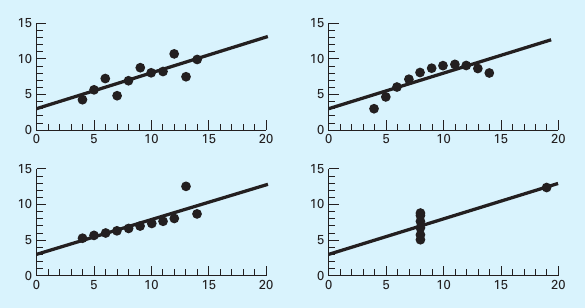
\includegraphics[width=1\linewidth]{fig_14_12}
	\caption{\textsf{Anscombe's four data sets along with the best-fit line, $y = 3 + 0.5x$.}}
	\label{fig:fig_14_12}
\end{figure}


\label{cha:cha_P_14_4}
\section{LINEARIZATION OF NONLINEAR RELATIONSHIPS}

Linear regression provides a powerful technique for fitting a best line to data. However, it is predicated on the fact that the relationship between the dependent and independent variables is linear. This is not always the case, and the first step in any regression analysis should be to plot and visually inspect the data to ascertain whether a linear model applies. In some cases, techniques such as polynomial regression, which is described in Chap. 15, are appropriate. For others, transformations can be used to express the data in a form that is compatible with linear regression.

One example is the \textit{exponential model}:

\begin{equation}
	\tag{14.22}
	y = a_1 e^{\beta_1 x}
\end{equation}

\noindent where $\alpha$ and $\beta_1$ are constants. This model is used in many fields of engineering and science to characterize quantities that increase (positive $\beta_1$) or decrease (negative $\beta_1$) at a rate that is directly proportional to their own magnitude. For example, population growth or radioactive decay can exhibit such behavior. As depicted in Fig. 14.13a, the equation represents a nonlinear relationship (for $\beta_1 \neq 0$) between $y$ and $x$.

Another example of a nonlinear model is the simple \textit{power equation:}

\begin{equation}
	\tag{14.23}
	y = a_2 x^{\beta_2}
\end{equation}

\noindent where $\alpha_2$ and $\beta_2$ are constant coefficients. This model has wide applicability in all fields of engineering and science. It is very frequently used to fit experimental data when the underlying model is not known. As depicted in Fig. 14.13b, the equation (for $\beta_2 \neq 0$) is nonlinear.

\begin{figure}[H]
	\centering
	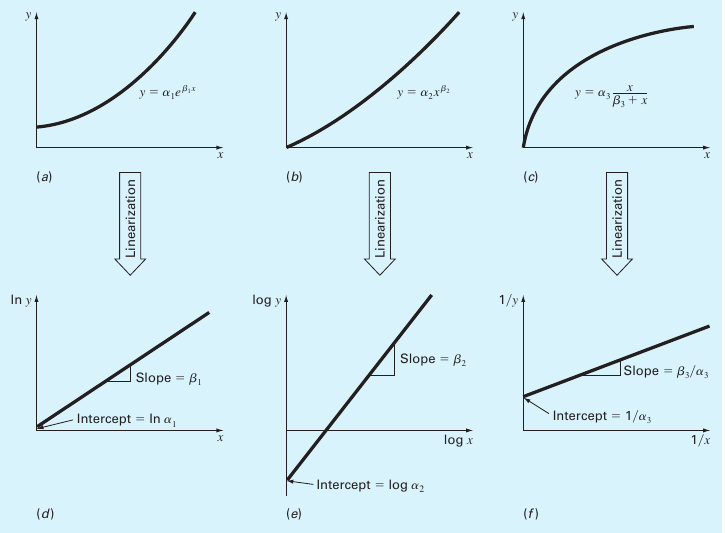
\includegraphics[width=1\linewidth]{fig_14_13}
	\caption{\textsf{(a) The exponential equation, (b) the power equation, and (c) the saturation-growth-rate equation. Parts (d), (e), and (f) are linearized versions of these equations that result from simple transformations.}}
	\label{fig:fig_14_13}
	\label{fig:fig_14_13a}
	\label{fig:fig_14_13b}
	\label{fig:fig_14_13c}
	\label{fig:fig_14_13d}
	\label{fig:fig_14_13e}
	\label{fig:fig_14_13f}
\end{figure}


A third example of a nonlinear model is the \textit{saturation-growth-rate equation}:

\begin{equation}
	\tag{14.24}
	y = \alpha_3 \frac{x}{\beta_3 + x}
\end{equation}

\noindent where $\alpha_3$ and $\beta_3$ are constant coefficients. This model, which is particularly well-suited for characterizing population growth rate under limiting conditions, also represents a nonlinear relationship between y and x (Fig. 14.13c) that levels off, or “saturates,” as $x$ increases. It has many applications, particularly in biologically related areas of both engineering and science.

Nonlinear regression techniques are available to fit these equations to experimental data directly. However, a simpler alternative is to use mathematical manipulations to trans form the equations into a linear form. Then linear regression can be employed to fit the equations to data.

For example, Eq. (14.22) can be linearized by taking its natural logarithm to yield

\begin{equation}
	\tag{14.25}
	\ln{y} = \ln{\alpha_1} + \beta_1 x
\end{equation}

\noindent Thus, a plot of $\ln{y}$ versus $x$ will yield a straight line with a slope of $\beta_1$ and an intercept of $\ln{\alpha_1}$ (Fig. 14.13d).

Equation (14.23) is linearized by taking its base-10 logarithm to give

\begin{equation} % Page 346
	\tag{14.26}
	\log y = \log \alpha_2 + \beta_2 \log x
\end{equation} 

\noindent Thus, a plot of log y versus log x will yield a straight line with a slope of $\beta_2$ and an intercept of $\log \alpha_2$ (Fig. 14.13e). Note that any base logarithm can be used to linearize this model. However, as done here, the base-10 logarithm is most commonly employed.

Equation (14.24) is linearized by inverting it to give

\begin{equation}
	\tag{14.27}
	\frac{1}{y} = \frac{1}{\alpha_3} + \frac{\beta_3}{\alpha_3} \frac{1}{x}
\end{equation}

\noindent Thus, a plot of $1/y$ versus $1/x$ will be linear, with a slope of $\beta_3 / \alpha_3$ and an intercept of $1 / \alpha_3$ (Fig. 14.13f).

In their transformed forms, these models can be fit with linear regression to evaluate the constant coefficients. They can then be transformed back to their original state and used for predictive purposes. The following illustrates this procedure for the power model.

\begin{example} Estimation of Errors for the Linear Least-Squares Fit

    \noindent\textbf{Problem Statement.}\quad CFit Eq. (14.23) to the data in Table 14.1 using a logarithmic transformation.

    \noindent\textbf{Solution.}\quad  The data can be set up in tabular form and the necessary sums computed as in Table 14.6.

	The means can be computed as
	
	\begin{equation}
		\notag
		\bar{x} = \frac{12.606}{8}=1.5757 \quad \bar{y} = \frac{20.515}{8} = 2.5644
	\end{equation}

	% TODO  table 14.6

	\begin{figure}[H]
		\centering
		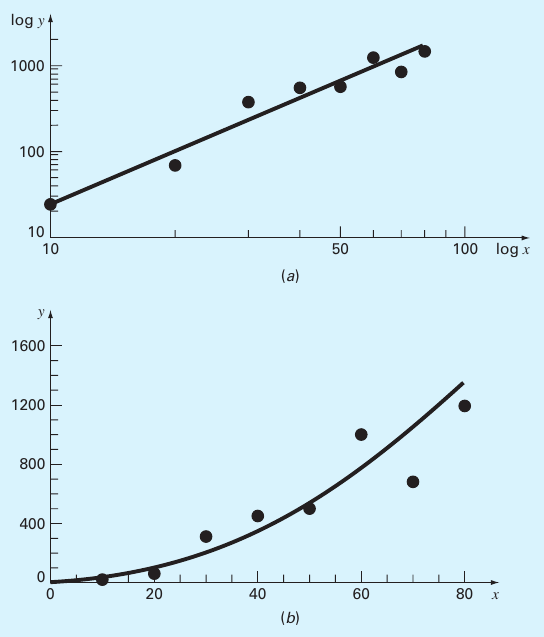
\includegraphics[width=1\linewidth]{fig_14_14}
		\caption{\textsf{Least-squares fit of a power model to the data from Table 14.1. (a) The fit of the transformed data.
		(b) The power equation fit along with the data.}}
		\label{fig:fig_14_14}
	\end{figure}

	\noindent The slope and the intercept can then be calculated with Eqs. (14.15) and (14.16) as

	\begin{equation}
		\notag
		a_1 = \frac{8(33.622) - 12.606(20.515)}{8(20.516) - (12.606)^2} = 1.9842
	\end{equation}

	\begin{equation}
		\notag
		a_0 = 2.5644 - 1.9842(1.5757) = -0.5620
	\end{equation}

	\noindent The least-squares fit is

	\begin{equation}
		\notag
		\log y = -0.5620 + 1.9842 \log x
	\end{equation}

	\noindent The fit, along with the data, is shown in Fig. 14.14a.

	We can also display the fit using the untransformed coordinates. To do this, the coefficients of the power model are determined as $\alpha_2 = 10^{-0.5620} = 0.2741$ and $\beta_2 = 1.9842$. Using force and velocity in place of $y$ and $x$, the least-squares fit is

	\begin{equation}
		\notag
		F = 0.2741 v ^ {1.9842}		
	\end{equation}

	\noindent This equation, along with the data, is shown in Fig. 14.14b.
\end{example}


The fits in Example 14.6 (Fig. 14.14) should be compared with the one obtained previously in Example 14.4 (Fig. 14.8) using linear regression on the untransformed data. Although both results would appear to be acceptable, the transformed result has the advantage that it does not yield negative force predictions at low velocities. Further, it is known from the discipline of fluid mechanics that the drag force on an object moving through a fluid is often well described by a model with velocity squared. Thus, knowledge from the field you are studying often has a large bearing on the choice of the appropriate model equation you use for curve fitting.


\label{cha:cha_P_14_4_1}
\subsection{General Comments on Linear Regression}

\noindent Before proceeding to curvilinear and multiple linear regression, we must emphasize the introductory nature of the foregoing material on linear regression. We have focused on the simple derivation and practical use of equations to fit data. You should be cognizant of the fact that there are theoretical aspects of regression that are of practical importance but are beyond the scope of this book. For example, some statistical assumptions that are inherent in the linear least-squares procedures are

\begin{enumerate}
	\item Each $x$ has a fixed value; it is not random and is known without error.
	\item The $y$ values are independent random variables and all have the same variance.
	\item The $y$ values for a given $x$ must be normally distributed.
\end{enumerate}

Such assumptions are relevant to the proper derivation and use of regression. For example, the first assumption means that (1) the $x$ values must be error-free and (2) the regression of $y$ versus $x$ is not the same as $x$ versus $y$. You are urged to consult other references such as Draper and Smith (1981) to appreciate aspects and nuances of regression that are beyond the scope of this book.

\label{cha:cha_P_14_5}
\section{COMPUTER APPLICATIONS}

\noindent Linear regression is so commonplace that it can be implemented on most pocket calculators. In this section, we will show how a simple M-file can be developed to determine the slope and intercept as well as to create a plot of the data and the best-fit line. We will also show how linear regression can be implemented with the built-in \texttt{polyfit} function.

\label{cha:cha_P_14_5_1}
\subsection{MATLAB M-file: \texttt{linregr}}
\noindent An algorithm for linear regression can be easily developed (Fig. 14.15). The required summations are readily computed with MATLAB's \texttt{sum} function. These are then used to compute the slope and the intercept with Eqs. (14.15) and (14.16). The routine displays the intercept and slope, the coefficient of determination, and a plot of the best-fit line along with the measurements.

A simple example of the use of this M-file would be to fit the force-velocity data analyzed in Example 14.4:

\begin{lstlisting}[numbers=none]
	>> x = [10 20 30 40 50 60 70 80];
	>> y = [25 70 380 550 610 1220 830 1450];
	>> linregr(x,y)
	r2 =
		0.8805
	ans =
		19.4702 -234.2857
\end{lstlisting}

\begin{figure}[H]
	\centering
	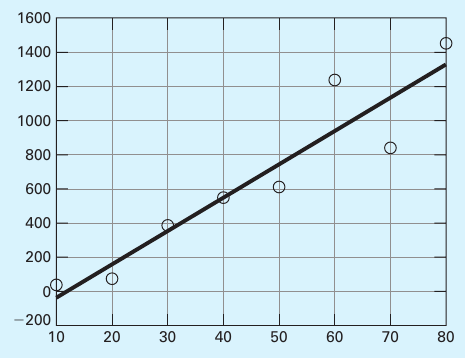
\includegraphics[width=1\linewidth]{fig_14_5_1_u_1}
\end{figure}

It can just as easily be used to fit the power model (Example 14.6) by applying the
\texttt{log10} function to the data as in

\begin{lstlisting}[numbers=none]
	>> linregr(log10(x),log10(y))
	r2 =
		0.9481
	ans =
		1.9842	-0.5620
\end{lstlisting}

\begin{figure}[H]
	\centering
	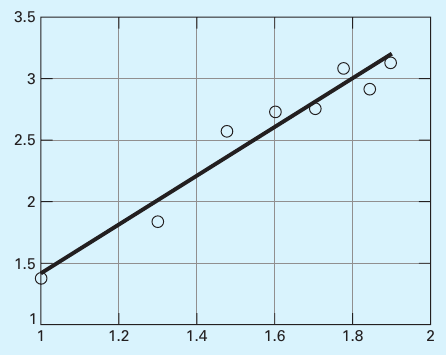
\includegraphics[width=1\linewidth]{fig_14_5_1_u_2}
\end{figure}

\begin{figure}[H]
	\centering
	\begin{lstlisting}[numbers=none]
		function [a, r2] = linregr(x,y)
		% linregr: linear regression curve fitting
		%	[a, r2] = linregr(x,y): Least squares fit of straight
		%		line to data by solving the normal equations

		% input:
		%	x = independent variable
		%	y = dependent variable
		% output:
		%	a = vector of slope, a(1), and intercept, a(2)
		%	r2 = coefficient of determination

		n = length(x);
		if length(y)~=n, error('x and y must be same length'); end
		x = x(:); y = y(:);
		% convert to column vectors
		sx = sum(x); sy = sum(y);
		sx2 = sum(x.*x); sxy = sum(x.*y); sy2 = sum(y.*y);
		a(1) = (n*sxy-sx*sy)/(n*sx2-sx^2);
		a(2) = sy/n-a(1)*sx/n;
		r2 = ((n*sxy-sx*sy)/sqrt(n*sx2-sx^2)/sqrt(n*sy2-sy^2))^2;
		% create plot of data and best fit line
		xp = linspace(min(x),max(x),2);
		yp = a(1)*xp+a(2);
		plot(x,y,'o',xp,yp)
		grid on
	\end{lstlisting}
	\caption{\textsf{An M-file to implement linear regression.}}
	\label{fig:fig_14_15}
\end{figure}

\label{cha:cha_P_14_5_2} %351
\subsection{MATLAB Functions: \texttt{polyfit} and \texttt{polyval}}

\noindent MATLAB has a built-in function \texttt{polyfit} that fits a least-squares \textit{n}th-order polynomial to data. It can be applied as in

\begin{lstlisting}[numbers=none]
>> p = polyfit(x, y, n)
\end{lstlisting}

\noindent where $x$ and $y$ are the vectors of the independent and the dependent variabless, respectively, and $n =$ the order of the polynomial. The function returns a vector $p$ containing the polynomial's coefficients. We should note that it represents the polynomial using decreasing powers of $x$ as in the following representation:

\begin{equation}
	\notag
	f(x) = p_1x^n + p_2x^{n-1} + \cdots + p_n x + p_{n + 1}
\end{equation}

Because a straight line is a first-order polynomial, \verb|polyfit(x,y,1)| will return the slope and the intercept of the best-fit straight line.

\begin{lstlisting}[numbers=none]
>> x = [10 20 30 40 50 60 70 80];
>> y = [25 70 380 550 610 1220 830 1450];
>> a = polyfit(x,y,1)
a =
	19.4702 -234.2857
\end{lstlisting}

\noindent Thus, the slope is 19.4702 and the intercept is -234.2857.

Another function, \texttt{polyval}, can then be used to compute a value using the coefficients. It has the general format:

\begin{lstlisting}[numbers=none]
>> y = polyval(p, x)
\end{lstlisting}

\noindent where $p =$ the polynomial coefficients, and $y =$ the best-fit value at $x$. For example,

\begin{lstlisting}[numbers=none]
>> y = polyval(a,45)
y =
	641.8750
\end{lstlisting}

\bigskip

% ENZYME KINETICS
\textbf{Background.} \textit{Enzymes} act as catalysts to speed up the rate of chemical reactions in living cells. In most cases, they convert one chemical, the \textit{substrate},into another, the \textit{product}. The \textit{Michaelis-Menten} equation is commonly used to describe such reactions:

\begin{equation}
	\tag{14.28}
	v = \frac{v_m[S]}{k_s + [S]}
\end{equation}

\noindent where $v =$ the initial reaction velocity, $v_m =$ the maximum initial reaction velocity, $[S] =$ substrate concentration, and $k_s =$ a half-saturation constant. As in Fig. 14.16, the equation describes a saturating relationship which levels off with increasing $[S]$. The graph also illustrates that the \textit{half-saturation constant} corresponds to the substrate concentration at which the velocity is half the maximum.

\begin{figure}[H] % Page 352
	\centering
	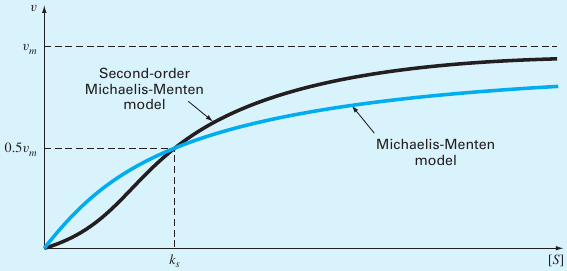
\includegraphics[width=1\linewidth]{fig_14_16}
	\caption{\textsf{Two versions of the Michaelis-Menten model of enzyme kinetics.}}
	\label{fig:fig_14_16}
\end{figure}

Although the Michaelis-Menten model provides a nice starting point, it has been refined and extended to incorporate additional features of enzyme kinetics. One simple extension involves so-called \textit{allosteric enzymes}, where the binding of a substrate molecule at one site leads to enhanced binding of subsequent molecules at other sites. For cases with two interacting bonding sites, the following second-order version often results in a better fit:

\begin{equation}
	\tag{14.29}
	v = \frac{v_m {[S]}^2}{k^2_s + {[S]}^2}
\end{equation}

\noindent This model also describes a saturating curve but, as depicted in Fig. 14.16, the squared concentrations tend to make the shape more \textit{sigmoid},or S-shaped.

Suppose that you are provided with the following data:
% todo this should be a table
\begin{lstlisting}[numbers=none] 
[S] 1.3  1.8  3    4.5   6     8    9
v   0.07 0.13 0.22 0.275 0.335 0.35 0.36
\end{lstlisting}

\noindent Employ linear regression to fit these data with linearized versions of Eqs. (14.28) and (14.29). Aside from estimating the model parameters, assess the validity of the fits with both statistical measures and graphs.

\textbf{Solution.} Equation (14.28), which is in the format of the saturation-growth-rate model (Eq. 14.24), can be linearized by inverting it to give (recall Eq. 14.27)

\begin{equation}
	\notag
	\frac{1}{v} = \frac{1}{v_m} + \frac{k_s}{v_m} \frac{1}{[S]}
\end{equation}

\noindent The \texttt{linregr} function from Fig. 14.15 can then be used to determine the least-squares fit:

\begin{lstlisting}[numbers=none] 
>> S=[1.3 1.8 3 4.5 6 8 9];
>> v=[0.07 0.13 0.22 0.275 0.335 0.35 0.36];
>> [a,r2]=linregr(1./S,1./v)
a =
16.4022
 0.1902
r2 =
0.9344
\end{lstlisting}

\noindent The model coefficients can then be calculated as

\begin{lstlisting}[numbers=none] 
>> vm=1/a(2)
vm =
5.2570
>> ks=vm*a(1)
ks =
86.2260
\end{lstlisting}

\noindent Thus, the best-fit model is

\begin{equation}
	\notag
	v = \frac{5.2570[S]}{86.2260 + [S]}
\end{equation}

Although the high value of $r^2$ might lead you to believe that this result is acceptable, inspection of the coefficients might raise doubts. For example, the maximum velocity (5.2570) is much greater than the highest observed velocity (0.36). In addition, the half-saturation rate (86.2260) is much bigger than the maximum substrate concentration (9).

The problem is underscored when the fit is plotted along with the data. Figure 14.17a shows the transformed version. Although the straight line follows the upward trend, the data clearly appear to be curved. When the original equation is plotted along with the data in the untransformed version (Fig. 14.17b), the fit is obviously unacceptable. The data are clearly leveling off at about 0.36 or 0.37. If this is correct, an eyeball estimate would suggest that $v_m$ should be about 0.36, and $k_s$ should be in the range of 2 to 3.

Beyond the visual evidence, the poorness of the fit is also reflected by statistics like the coefficient of determination. For the untransformed case, a much less acceptable result of $r^2 = 0.6406$ is obtained.


The foregoing analysis can be repeated for the second-order model. Equation (14.28) can also be linearized by inverting it to give

\begin{equation}
	\notag
	\frac{1}{v} = \frac{1}{v_m} + \frac{k^2_s}{v_m} \frac{1}{[S]^2}
\end{equation}

The \texttt{linregr} function from Fig. 14.15 can again be used to determine the least-squares fit:

\begin{lstlisting}[numbers=none] 
>> [a,r2]=linregr(1./S.^2,1./v)
a =
19.3760
 2.4492
r2 =
0.9929
\end{lstlisting}

% Page 354
\begin{figure}[H] 
	\centering
	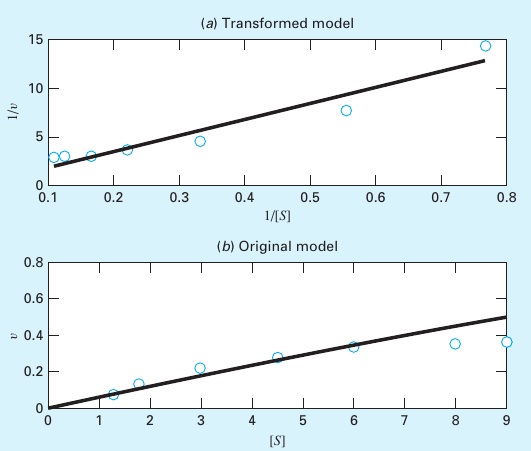
\includegraphics[width=1\linewidth]{fig_14_17}
	\caption{\textsf{Plots of least-squares fit (line) of the Michaelis-Menten model along with data (points). The plot in (a) shows the transformed fit, and (b) shows how the fit looks when viewed in the untransformed, original form.}}
	\label{fig:fig_14_17}
\end{figure}

\noindent The model coefficients can then be calculated as

\begin{lstlisting}[numbers=none] 
>> vm=1/a(2)
vm =
0.4083
>> ks=sqrt(vm*a(1))
ks =
2.8127
\end{lstlisting}

\noindent Substituting these values into Eq. (14.29) gives

\begin{equation}
	\notag
	v = \frac{0.4083[S]^2}{7.911 + [S]^2}
\end{equation}

Although we know that a high $r^2$ does not guarantee of a good fit, the fact that it is very high (0.9929) is promising. In addition, the parameters values also seem consistent with the trends in the data; that is, the $k_m$ is slightly greater than the highest observed velocity and the half-saturation rate is lower than the maximum substrate concentration (9).

\begin{figure}[H] 
	\centering
	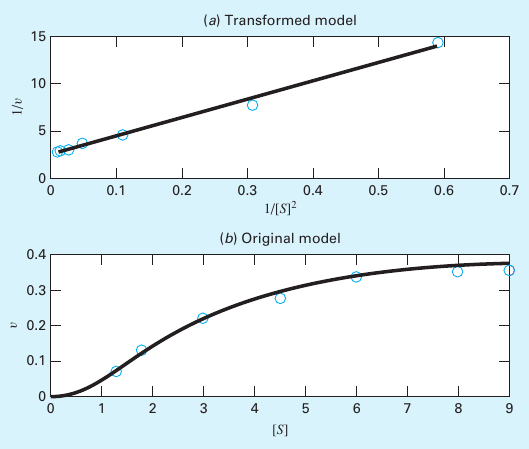
\includegraphics[width=1\linewidth]{fig_14_18}
	\caption{\textsf{Plots of least-squares fit (line) of the second-order Michaelis-Menten model along with data (points). The plot in (a) shows the transformed fit, and (b) shows the untransformed, original form.}}
	\label{fig:fig_14_18}
\end{figure}

The adequacy of the fit can be assessed graphically. As in Fig. 14.18a, the transformed results appear linear. When the original equation is plotted along with the data in the untransformed version (Fig. 14.18b), the fit nicely follows the trend in the measurements. Beyond the graphs, the goodness of the fit is also reflected by the fact that the coefficient of determination for the untransformed case can be computed as $r^2 = 0.9896$.

Based on our analysis, we can conclude that the second-order model provides a good fit of this data set. This might suggest that we are dealing with an allosteric enzyme. 

Beyond this specific result, there are a few other general conclusions that can be drawn from this case study. First, we should never solely rely on statistics such as $r^2$ as the sole basis of assessing goodness of fit. Second, regression equations should always be assessed graphically. And for cases where transformations are employed, a graph of the untransformed model and data should always be inspected. 

Finally, although transformations may yield a decent fit of the transformed data, this does not always translate into an acceptable fit in the original format. The reason that this might occur is that minimizing squared residuals of transformed data is not the same as for the untransformed data. Linear regression assumes that the scatter of points around the best-fit line follows a Gaussian distribution,  and that the standard deviation is the same at every value of the dependent variable. These assumptions are rarely true after transforming data. 

As a consequence of the last conclusion, some analysts suggest that rather than using linear transformations, nonlinear regression should be employed to fit curvilinear data. In this approach, a best-fit curve is developed that directly minimizes the untransformed residuals. We will describe how this is done in Chap. 15.


\bigskip
\noindent\textbf{PROBLEMS}\\

\begin{multicols}{2}
    \noindent\textbf{14.1} Given the data

	\noindent \begin{tabular}{ c c c c c }
		0.90 & 1.42 & 1.30 & 1.55 & 1.63 \\
		1.32 & 1.35 & 1.47 & 1.95 & 1.66 \\
		1.96 & 1.47 & 1.92 & 1.35 & 1.05 \\
		1.85 & 1.74 & 1.65 & 1.78 & 1.71 \\
		2.29 & 1.82 & 2.06 & 2.14 & 1.27
	\end{tabular}

	\noindent Determine \textbf{(a)} the mean, \textbf{(b)} median, \textbf{(c)} mode, \textbf{(d)} range,
	\textbf{(e)} standard deviation, \textbf{(f)} variance, and \textbf{(g)} coefficient of
	variation.	


	\noindent\textbf{14.2}  Construct a histogram from the data from Prob. 14.1. Use a range from 0.8 to 2.4 with intervals of 0.2.

	\noindent\textbf{14.3} Given the data

	\noindent \begin{tabular}{c c c c c c c}
		29.65 & 28.55 & 28.65 & 30.15 & 29.35 & 29.75 & 29.25 \\
		30.65 & 28.15 & 29.85 & 29.05 & 30.25 & 30.85 & 28.75 \\
		29.65 & 30.45 & 29.15 & 30.45 & 33.65 & 29.35 & 29.75 \\
		31.25 & 29.45 & 30.15 & 29.65 & 30.55 & 29.65 & 29.25
	\end{tabular}

	\noindent Determine \textbf{(a)} the mean, \textbf{(b)} median, \textbf{(c)} mode, \textbf{(d)} range,
	\textbf{(e)} standard deviation, \textbf{(f)} variance, and \textbf{(g)} coefficient of
	variation.
	\textbf{(h)} Construct a histogram. Use a range from 28 to 34 with
	increments of 0.4.
	\textbf{(i)} Assuming that the distribution is normal, and that your
	estimate of the standard deviation is valid, compute the
	range (i.e., the lower and the upper values) that encompasses 68\% of the readings. Determine whether this is a
	valid estimate for the data in this problem.

	\noindent\textbf{14.4} Using the same approach as was employed to derive
	Eqs. (14.15) and (14.16), derive the least-squares fit of the
	following model:

	$$y = a_1 x + e$$

	\noindent That is, determine the slope that results in the leastsquares fit for a straight line with a zero intercept. Fit the following data with this model and display the result graphically.

	\noindent \begin{tabular}{c c c c c c c c c c }
	 	\textbf{x} & 2 & 4 & 6 & 7 & 10 & 11 & 		14 & 		17 & 		20 \\
	  	\textbf{y} & 4 & 5 & 6 & 5 & 8 & 8 & 6 & 9 & 		12
	\end{tabular}

	\noindent\textbf{14.5} Use least-squares regression to fit a straight line to

	\noindent \begin{tabular}{c c c c c c c c c c c  }
 		x & 0 & 2 & 4 & 6 & 9 & 11 & 12 & 15 & 17 & 19 \\
 		y & 5 & 6 & 7 & 6 & 9 & 8 & 8 & 10 & 12 & 12
   	\end{tabular}

   	\noindent Along with the slope and intercept, compute the standard
	   error of the estimate and the correlation coefficient. Plot the
	   data and the regression line. Then repeat the problem, but
	   regress $x$ versus $y$ - that is, switch the variables. Interpret
	   your results.

	\noindent\textbf{14.6} Fit a power model to the data from Table 14.1, but use
	natural logarithms to perform the transformations.

	\noindent\textbf{14.7} The following data were gathered to determine the
	relationship between pressure and temperature of a fixed
	volume of 1 kg of nitrogen. The volume is 10 m$^3$.

	\noindent \begin{tabular}{l c c c c c c c c c c  }
		\textbf{T, $^\circ$C} & -40 & 0 & 40 & 80 & 120 & 160 \\
		\textbf{p, N/m$^2$} & 6900 & 8100 & 9350 & 10,500 & 11,700 & 12,800
  	\end{tabular}

	\noindent Employ the ideal gas law $pV = nRT$ to determine $R$ on the
	basis of these data. Note that for the law, $T$ must be expressed
	in kelvins.

	\noindent\textbf{14.8} Beyond the examples in Fig. 14.13, there are other
	models that can be linearized using transformations. For
	example,

	$$y = a_4 x e^{\beta_4 x}$$

	\noindent Linearize this model and use it to estimate $\alpha_4$ and $\beta_4$ based
	on the following data. Develop a plot of your fit along with
	the data.

	\noindent \begin{tabular}{c c c c c c c c c c}
		\textbf{x} & 0.1 & 0.2 & 0.4 & 0.6 & 0.9 & 1.3 & 1.5 & 1.7 & 1.8 \\
		\textbf{y} & 0.75 & 1.25 & 1.45 & 1.25 & 0.85 & 0.55 & 0.35 & 0.28 & 0.18	
  	\end{tabular}

	\noindent\textbf{14.9} The concentration of \textit{E. coli} bacteria in a swimming
	area is monitored after a storm:

	\noindent \begin{tabular}{l c c c c c c}
		\textbf{t (hr)} & 4 & 8 & 12 & 16 & 20 & 24 \\
		\textbf{c (CFU/100 mL)} & 1600 & 1320 & 1000 & 890 & 650 & 560
  	\end{tabular}

	\noindent The time is measured in hours following the end of the storm
	and the unit CFU is a ``colony forming unit.'' Use this data to
	estimate \textbf{(a)} the concentration at the end of the storm ($t = 0$)
	and \textbf{(b)} the time at which the concentration will reach
	200 CFU/100 mL. Note that your choice of model should
	be consistent with the fact that negative concentrations are
	impossible and that the bacteria concentration always decreases with time.

	\noindent\textbf{14.10} Rather than using the base-$e$ exponential model
	(Eq. 14.22), a common alternative is to employ a base-10
	model:

	$$y = \alpha_5 10^{\beta_5 x}$$

	\noindent When used for curve fitting, this equation yields identical
	results to the base-$e$ version, but the value of the exponent
	parameter ($\beta_5$) will differ from that estimated with Eq.14.22
	($\beta_1$). Use the base-10 version to solve Prob. 14.9. In addition, develop a formulation to relate $\beta_1$ to $\beta_5$ .

	\noindent\textbf{14.11} Determine an equation to predict metabolism rate as a
	function of mass based on the following data. Use it to predict the metabolism rate of a 200-kg tiger.

	\noindent \begin{tabular}{l c c }
		\textbf{Animal} & \textbf{Mass (kg)} & \textbf{Metabolism (watts)} \\
		\hline
		Cow &  400 &  270 \\
		Human &  70 &  82 \\ 
		Sheep &  45 &  50 \\ 
		Hen &  2 &  4.8 \\ 
		Rat &  0.3 &  1.45 \\ 
		Dove &  0.16 &  0.97
  	\end{tabular}

	\noindent\textbf{14.12} On average, the surface area $A$ of human beings is
	related to weight $W$ and height $H$. Measurements on a number of individuals of height 180 cm and different weights
	(kg) give values of $A$ (m$^2$) in the following table:

	\noindent \begin{tabular}{l c c c c c c c c c}
		\textbf{W (kg)} & 70 & 75 & 77 & 80 & 82 & 84 & 87 & 90 \\
		\textbf{A (m2)} & 2.10 & 2.12 & 2.15 & 2.20 & 2.22 & 2.23 & 2.26 & 2.30 &
  	\end{tabular}

	\noindent Show that a power law $A = aW^b$ fits these data reasonably
	well. Evaluate the constants $a$ and $b$, and predict what the
	surface area is for a 95-kg person.

	\noindent\textbf{14.13} Fit an exponential model to

	\noindent \begin{tabular}{l c c c c c c }
		\textbf{x} & 0.4 & 0.8 & 1.2 & 1.6 & 2 & 2.3 \\
		\textbf{y} & 800 & 985 & 1490 & 1950 & 2850 & 3600
  	\end{tabular}

	\noindent Plot the data and the equation on both standard and semilogarithmic graphs with the MATLAB \texttt{subplot} function.

	\noindent\textbf{14.14} An investigator has reported the data tabulated below
	for an experiment to determine the growth rate of bacteria
	$k$ (per d) as a function of oxygen concentration $c$ (mg/L). It
	is known that such data can be modeled by the following
	equation:

	$$k = \frac{k_{\text{max}} c^2}{c_s + c^2}$$

	\noindent where $c_s$ and $k_{\text{max}}$ are parameters. Use a transformation to
	linearize this equation. Then use linear regression to estimate $c_s$ and $k_{\text{max}}$ and predict the growth rate at $c$ = 2 mg/L.

	\noindent \begin{tabular}{l c c c c c}
		\textbf{c} & 0.5 & 0.8 & 1.5 & 2.5 \\
		\textbf{k} & 1.1 & 2.5 & 5.3 & 7.6 & 8.9
  	\end{tabular}

	\noindent\textbf{14.15} Develop an M-file function to compute descriptive
	statistics for a vector of values. Have the function determine
	and display number of values, mean, median, mode, range,
	standard deviation, variance, and coefficient of variation. In
	addition, have it generate a histogram. Test it with the data
	from Prob. 14.3.

	\noindent\textbf{14.16}  Modify the \texttt{linregr} function in Fig. 14.15 so that it
	\textbf{(a)} computes and returns the standard error of the estimate,
	and \textbf{(b)} uses the \texttt{subplot} function to also display a plot of
	the residuals (the predicted minus the measured $y$) versus $x$.

	\noindent\textbf{14.17} Develop an M-file function to fit a power model.
	Have the function return the best-fit coefficient $\alpha_2$ and
	power $\beta_2$ along with the $r^2$ for the untransformed model. In
	addition, use the \texttt{subplot} function to display graphs of both
	the transformed and untransformed equations along with the
	data. Test it with the data from Prob. 14.11.

	\noindent\textbf{14.18} The following data show the relationship between the
	viscosity of SAE 70 oil and temperature. After taking the log
	of the data, use linear regression to find the equation of the
	line that best fits the data and the $r^2$ value.

	\noindent \begin{tabular}{l c c c c}
		\textbf{Temperature, $^\circ$C} & 26.67 & 93.33 & 148.89 & 315.56 \\
		\textbf{Viscosity, $\mu$, N $\cdot$ s/m$^2$} & 1.35 & 0.085 & 0.012 & 0.00075
  	\end{tabular}

	\noindent\textbf{14.19} You perform experiments and determine the following values of heat capacity $c$ at various temperatures $T$ for a gas:

	\noindent \begin{tabular}{l c c c c c c}
		\textbf{T} & -50 & -30 & 0 & 60 & 90 & 110 \\
		\textbf{c} & 1250 & 1280 & 1350 & 1480 & 1580 & 1700
  	\end{tabular}

	\noindent Use regression to determine a model to predict $c$ as a function of $T$.

	\noindent\textbf{14.20} It is known that the tensile strength of a plastic increases as a function of the time it is heat treated. The following data are collected:

	\noindent \begin{tabular}{l c c c c c c c c c c}
		\textbf{Time} & 10 & 15 & 20 & 25 & 40 & 50 & 55 & 60 & 75 \\
		\textbf{Tensile Strength} & 5 & 20 & 18 & 40 & 33 & 54 & 70 & 60 & 78
  	\end{tabular}

	\noindent \textbf{(a)} Fit a straight line to these data and use the equation to
	determine the tensile strength at a time of 32 min.


	\noindent \textbf{(b)} Repeat the analysis but for a straight line with a zero
	intercept.

	\noindent\textbf{14.21}  The following data were taken from a stirred tank reactor for the reaction $A \rightarrow B$. Use the data to determine the
	best possible estimates for $k_{01}$ and $E_1$ for the following
	kinetic model:

	$$- \frac{d A}{d t} = k _{01} e^{-E_1 / RT} A$$

	\noindent where $R$ is the gas constant and equals 0.00198 kcal/mol/K.

	\noindent \begin{tabular}{l c c c c c c c c}
		\textbf{-dA/dt (moles/L/s)} & 460 & 960 & 2485 & 1600 & 1245 \\ 
		\textbf{A (moles/L)} & 200 & 150 & 50 & 20 & 10 \\
		\textbf{T (K)} & 280 & 320 & 450 & 500 & 550
	\end{tabular}

	\noindent\textbf{14.22} Concentration data were collected at 15 time points
	for the polymerization reaction:

	$$x A + y B \rightarrow A_x B_y$$

	\noindent We assume the reaction occurs via a complex mechanism
	consisting of many steps. Several models have been hypothesized, and the sum of the squares of the residuals had been
	calculated for the fits of the models of the data. The results are shown below. Which model best describes the data (statistically)? Explain your choice.


	\noindent \begin{tabular}{l c c c}
		 & \textbf{Model A} & \textbf{Model B} & \textbf{Model C} \\
		\hline
		\textbf{S$_r$} & 135 & 105 & 100 \\
		\textbf{Number of Model} \\
		\textbf{Parameters Fit} & 2 & 3 & 5
  	\end{tabular}

	\noindent\textbf{14.23} Below are data taken from a batch reactor of bacterial
	growth (after lag phase was over). The bacteria are allowed
	to grow as fast as possible for the first 2.5 hours, and then
	they are induced to produce a recombinant protein, the production of which slows the bacterial growth significantly.
	The theoretical growth of bacteria can be described by

	$$\frac{d X}{dt} = \mu X$$

	\noindent where $X$ is the number of bacteria, and $\mu$ is the specific
	growth rate of the bacteria during exponential growth. Based
	on the data, estimate the specific growth rate of the bacteria
	during the first 2 hours of growth and during the next 4 hours
	of growth.

	\noindent \begin{tabular}{l c c c c c c c c}
		\textbf{Time,} \\
		\textbf{h} &  0 &  1 &  2 &  3 &  4 &  5 &  6 \\
		\textbf{[Cells],} \\
		\textbf{g/L} & 0.100 & 0.335 & 1.102 & 1.655 & 2.453 & 3.702 & 5.460
	\end{tabular}

	\noindent\textbf{14.24} A transportation engineering study was conducted to
	determine the proper design of bike lanes. Data were gathered on bike-lane widths and average distance between bikes
	and passing cars. The data from 9 streets are

	\noindent \begin{tabular}{l c c c c c c c c c c c c}
		\textbf{Distance, m} & 2.4 & 1.5 & 2.4 & 1.8 & 1.8 & 2.9 & 1.2 & 3 & 1.2 \\
		\textbf{Lane Width, m} & 2.9 & 2.1 & 2.3 & 2.1 & 1.8 & 2.7 & 1.5 & 2.9 & 1.5
	\end{tabular}

	\noindent \textbf{(a)} Plot the data.

	\noindent \textbf{(b)} Fit a straight line to the data with linear regression. Addthis line to the plot.

	\noindent \textbf{(c)} If the minimum safe average distance between bikes and passing cars is considered to be 1.8 m, determine the corresponding minimum lane width.

	\noindent\textbf{14.25}  In water-resources engineering, the sizing of reser	voirs depends on accurate estimates of water flow in the
	river that is being impounded. For some rivers, long-term
	historical records of such flow data are difficult to obtain. In
	contrast, meteorological data on precipitation are often
	available for many years past. Therefore, it is often useful to determine a relationship between flow and precipitation.
	This relationship can then be used to estimate flows for
	years when only precipitation measurements were made.
	The following data are available for a river that is to be
	dammed:

	\noindent \begin{tabular}{l c c c c c c c c c c}
		\textbf{Precip.,} \\
		\textbf{cm/yr} & 88.9 & 108.5 & 104.1 & 139.7 & 127 & 94 & 116.8 & 99.1 \\
		\textbf{Flow,} \\
		\textbf{m$^3$/s} & 14.6 & 16.7 & 15.3 & 23.2 & 19.5 & 16.1 & 18.1 & 16.6
	\end{tabular}	

		\noindent \textbf{(a)} Plot the data.

	\noindent \textbf{(b)} Fit a straight line to the data with linear regression.
Superimpose this line on your plot.

	\noindent \textbf{(c)} Use the best-fit line to predict the annual water flow if
the precipitation is 120 cm.

	\noindent \textbf{(d)} If the drainage area is 1100 km$^2$, estimate what fraction
of the precipitation is lost via processes such as evaporation, deep groundwater infiltration, and consumptive
use.

	\noindent\textbf{14.26}  The mast of a sailboat has a cross-sectional area of
	10.65 cm$^2$ and is constructed of an experimental aluminum
	alloy. Tests were performed to define the relationship between stress and strain. The test results are

	\noindent \begin{tabular}{l c c c c c c c c c c}
		\textbf{Strain,} \\
		\textbf{cm/cm} & 0.0032 & 0.0045 & 0.0055 & 0.0016 & 0.0085 & 0.0005 \\
		\textbf{Stress,} \\
		\textbf{N/cm$^2$} & 4970 & 5170 & 5500 & 3590 & 6900 & 1240
	\end{tabular}

	\noindent The stress caused by wind can be computed as $F/A_c$ where $F$ = force in the mast and $A_c$ = mast's cross-sectional area. This value can then be substituted into Hooke's law to determine the mast's deflection, $\Delta L$ = strain $\times L$, where $L$ = the mast's length. If the wind force is 25,000 N, use the data to estimate the deflection of a 9-m mast.

	\noindent\textbf{14.27} The following data were taken from an experiment
	that measured the current in a wire for various imposed voltages:

	\noindent \begin{tabular}{l c c c c c c c c c c}
		\textbf{$V$, V} & 2 & 3 & 4 & 5 & 7 & 10 \\
		\textbf{$i$, A} & 5.2 & 7.8 & 10.7 & 13 & 19.3 & 27.5
	\end{tabular}

	\noindent \textbf{(a)} On the basis of a linear regression of this data, determine
current for a voltage of 3.5 V. Plot the line and the data
and evaluate the fit.

\noindent \textbf{(b)} Redo the regression and force the intercept to be zero.

	\noindent\textbf{14.28} An experiment is performed to determine the \% elongation of electrical conducting material as a function of temperature. The resulting data are listed below. Predict the \%
	elongation for a temperature of $400^\circ$C.

	\noindent \begin{tabular}{l c c c c c c c c c c}
		\textbf{Temperature, $^\circ$C} & 200 & 250 & 300 & 375 & 425 & 475 & 600 \\
		\textbf{\% Elongation} & 7.5 & 8.6 & 8.7 & 10 & 11.3 & 12.7 & 15.3
	\end{tabular}

	\noindent\textbf{14.29} The population $p$ of a small community on the outskirts of a city grows rapidly over a 20-year period:

	\noindent \begin{tabular}{l c c c c c c c c c c}
		\textbf{t} & 0 & 5 & 10 & 15 & 20 \\
		\textbf{p} & 100 & 200 & 450 & 950 & 2000
	\end{tabular}

	\noindent As an engineer working for a utility company, you must
	forecast the population 5 years into the future in order to an	ticipate the demand for power. Employ an exponential
	model and linear regression to make this prediction.

	\noindent\textbf{14.30} The velocity u of air flowing past a flat surface is
	measured at several distances y away from the surface. Fit a
	curve to this data assuming that the velocity is zero at the
	surface ($y = 0$). Use your result to determine the shear stress
	($du/dy$) at the surface.

	\noindent \begin{tabular}{l c c c c c c c c c c}
		\textbf{$y$, m} & 0.002 & 0.006 & 0.012 & 0.018 & 0.024 \\
		\textbf{$u$, m/s} & 0.287 & 0.899 & 1.915 & 3.048 & 4.299
	\end{tabular}

	\noindent\textbf{14.31} \textit{Andrade's equation} has been proposed as a model of the effect of temperature on viscosity:

	$$ \mu = De^{B/T_a}$$

	\noindent where $\mu$ = dynamic viscosity of water ($10^{-3}$ N$\cdot$s/m$^2$), $T_a$ = absolute temperature (K), and $D$ and $B$ are parameters. Fit this model to the following data for water:

	\noindent \begin{tabular}{l c c c c c c c c c c}
		\textbf{T} & 0 & 5 & 10 & 20 & 30 & 40 \\
		\textbf{$\mu$} & 1.787 & 1.519 & 1.307 & 1.002 & 0.7975 & 0.6529
	\end{tabular}

	\noindent\textbf{14.32} Perform the same computation as in Example 14.2,
	but in addition to the drag coefficient, also vary the mass
	uniformly by $\pm 10\%$.

	\noindent\textbf{14.33} Perform the same computation as in Example 14.3,
	but in addition to the drag coefficient, also vary the mass
	normally around its mean value with a coefficient of variation of 5.7887\%.

	\noindent\textbf{14.34}  Manning's formula for a rectangular channel can be
	written as

	$$Q = \frac{1}{n_m} \frac{(BH) ^ {5/3}}{(B+2H) ^ {2/3}} \sqrt{S}$$

	\noindent where $Q$ = flow (m$^3$/s), $n_m$ = a roughness coefficient, $B$ =
	width (m), $H$ = depth (m), and $S$ = slope. You are applying
	this formula to a stream where you know that the width = 20 m
	and the depth = 0.3 m. Unfortunately, you know the roughness and the slope to only a $\pm 10\%$ precision. That is, you
	know that the roughness is about 0.03 with a range from 0.027
	to 0.033 and the slope is 0.0003 with a range from 0.00027
	to 0.00033. Assuming uniform distributions, use a Monte
	Carlo analysis with $n$ = 10,000 to estimate the distribution
	of flow.

	\noindent\textbf{14.35} A Monte Carlo analysis can be used for optimization.
	For example, the trajectory of a ball can be computed with

	\begin{equation}
		\tag{P14.35}
		y = (\tan \theta_0)x - \frac{g}{2 v^2_0 \cos ^2 \theta_0} x^2 + y_0
	\end{equation}

	\noindent where $y$ = the height (m), $\theta_0$ = the initial angle (radians),
	$v_0$ = the initial velocity (m/s), $g$ = the gravitational constant =
	9.81 m/s$^2$, and $y_0$ = the initial height (m). Given $y_0$ = 1 m,
	$v_0$ = 25 m/s, and $\theta_0 = 50^\circ$, determine the maximum height
	and the corresponding $x$ distance (\textbf{a}) analytically with calculus and (\textbf{b}) numerically with Monte Carlo simulation. For
	the latter, develop a script that generates a vector of 10,000
	uniformly-distributed values of $x$ between 0 and 60 m. Use
	this vector and Eq. P14.35 to generate a vector of heights.
	Then, employ the \texttt{max} function to determine the maximum
	height and the associated $x$ distance.
\end{multicols}

\label{cha:cha_P_15} %351
\chapter{General Linear Least-Squares and Nonlinear Regression}
\textbf{CHAPTER OBJECTIVES}

\noindent This chapter takes the concept of fitting a straight line and extends it to (a) fitting a polynomial and (b) fitting a variable that is a linear function of two or more independent variables. We will then show how such applications can be generalized and applied to a broader group of problems. Finally, we will illustrate how optimization techniques can be used to implement nonlinear regression. Specific objectives and topics covered are

\begin{itemize}
	\item Knowing how to implement polynomial regression.
	\item Knowing how to implement multiple linear regression. %why FIXME
	\item Understanding the formulation of the general linear least-squares model.
	\item Understanding how the general linear least-squares model can be solved with MATLAB using either the normal equations or left division.
	\item Understanding how to implement nonlinear regression with optimization techniques.
\end{itemize}


\label{cha:cha_P_15_1}
\section{POLYNOMIAL REGRESSION}
\noindent In Chap.14, a procedure was developed to derive the equation of a straight line using the least-squares criterion. Some data, although exhibiting a marked pattern such as seen in Fig. 15.1, are poorly represented by a straight line. For these cases, a curve would be better suited to fit the data. As discussed in Chap. 14, one method to accomplish this objective is to use transformations. Another alternative is to fit polynomials to the data using \emph{polynomial regression}.

The least-squares procedure can be readily extended to fit the data to a higher-orderpolynomial. For example,  suppose that we fit a second-order polynomial or quadratic:

\begin{equation}
	\tag{15.1}
	y = a_0 + a_1x + a_2x^2 + e
\end{equation}

\begin{wrapfigure}{l}{0.25\textwidth}
    \centering
    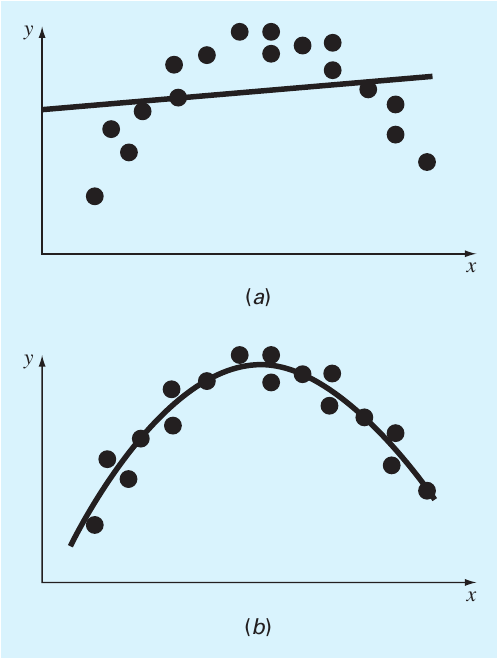
\includegraphics[width=0.25\textwidth]{fig_15_1}
   \caption{\textsf{(a) Data that are ill-suited for linear least-squares regression. (b) Indication that a parabola is preferable.}}
   \label{fig:fig_15_1}
\end{wrapfigure}

\noindent For this case the sum of the squares of the residuals is

\begin{equation}
	\tag{15.2}
	S_r = \sum^n_{i=1}(y_i - a_0 - a_1x_i - a_2x^2_i)^2
\end{equation}

To generate the least-squares fit, we take the derivative of Eq. (15.2) with respect to each of the unknown coefficients of the polynomial, as in

\begin{equation}
	\notag
	\frac{\partial S_r}{\partial a_0} = -2 \sum (y_i -a_0 -a_1x_i - a_2x_i^2)
\end{equation}

\begin{equation}
	\notag
	\frac{\partial S_r}{\partial a_1} = -2 \sum x_i (y_i -a_0 -a_1x_i - a_2x_i^2)
\end{equation}

\begin{equation}
	\notag
	\frac{\partial S_r}{\partial a_2} = -2 \sum x_i^2 (y_i -a_0 -a_1x_i - a_2x_i^2)
\end{equation}

\noindent These equations can be set equal to zero and rearranged to develop the following set of normal equations:

\begin{equation}
	\notag
	(n)a_0 + (\sum x_i) a_1 + (\sum x^2_i) a_2 = \sum y_i
\end{equation}

\begin{equation}
	\notag
	(\sum x_i)a_0 + (\sum x_i ^ 2) a_1 + (\sum x^3_i) a_2 = \sum x_i y_i
\end{equation}

\begin{equation}
	\notag
	(\sum x_i^2)a_0 + (\sum x_i ^ 3) a_1 + (\sum x^4_i) a_2 = \sum x_i^2 y_i
\end{equation}

\noindent where all summations are from $i = 1$ through $n$. Note that the preceding three equations are linear and have three unknowns: $a_0$ , $a_1$, and $a_2$. The coefficients of the unknowns can be calculated directly from the observed data.

For this case, we see that the problem of determining a least-squares second-order polynomial is equivalent to solving a system of three simultaneous linear equations. The two-dimensional case can be easily extended to an $m$th-order polynomial as in

\begin{equation}
	\notag
	y = a_0 + a_1 x + a_2 x^2 + \cdots + a_m x^m + e
\end{equation}

The foregoing analysis can be easily extended to this more general case. Thus, we can recognize that determining the coefficients of an $m$th-order polynomial is equivalent to solving a system of $m + 1$ simultaneous linear equations. For this case, the standard error is formulated as

\begin{equation}
	\tag{15.3}
	s_{y/x} = \sqrt{\frac{S_r}{n - (m + 1)}}
\end{equation}

This quantity is divided by $n - (m + 1)$ because $(m + 1)$ data-derived coefficients - $a_0, a_1, ..., a_m$ - were used to compute $S_r$; thus, we have lost $m + 1$ degrees of freedom. In addition to the standard error, a coefficient of determination can also be computed for polynomial regression with Eq. (14.20).

% TODO EXAMPLE 15.1

\label{cha:cha_P_15_2} % 365
\section{MULTIPLE LINEAR REGRESSION}

\noindent Another useful extension of linear regression is the case where $y$ is a linear function of two or more independent variables. For example, $y$ might be a linear function of $x_1$ and $x_2$, as in

\begin{equation}
	\notag
	y = a_0 + a_1x_1 + a_2x_2+e
\end{equation}

\noindent Such an equation is particularly useful when fitting experimental data where the variable being studied is often a function of two other variables. For this two-dimensional case, the regression ``line'' becomes a ``plane'' (Fig. 15.3).

As with the previous cases, the "best" values of the coefficients are determined by formulating the sum of the squares of the residuals:

\begin{equation}
	\tag{15.4}
	S_r = \sum_{i=1}^n (y_i - a_0 - a_1x_{1,i} - a_2x_{2,i})^2
\end{equation}

\noindent and differentiating with respect to each of the unknown coefficients:

\begin{equation}
	\notag
	\frac{\partial S_r}{\partial a_0} = -2 \sum (y_i -a_0 -a_1x_{1,i} - a_2x_{2,i}^2)
\end{equation}

\begin{equation}
	\notag
	\frac{\partial S_r}{\partial a_1} = -2 \sum x_{1,i} (y_i -a_0 -a_1x_{1,i} - a_2x_{2,i}^2)
\end{equation}

\begin{equation}
	\notag
	\frac{\partial S_r}{\partial a_2} = -2 \sum x_{2,i}^2 (y_i -a_0 -a_1x_{1,i} - a_2x_{2,i}^2)
\end{equation}

\begin{wrapfigure}{l}{0.25\textwidth}
    \centering
    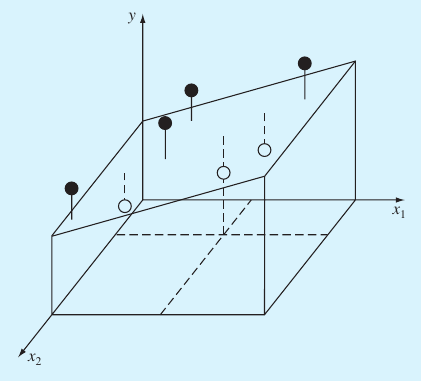
\includegraphics[width=0.25\textwidth]{fig_15_3}
   \caption{\textsf{Graphical depiction of multiple linear regression where y is a linear function of $x_1$ and $x_2$.}}
   \label{fig:fig_15_3}
\end{wrapfigure}

\noindent The coefficients yielding the minimum sum of the squares of the residuals are obtained by setting the partial derivatives equal to zero and expressing the result in matrix form as 

\begin{equation} % 366
	\tag{15.5}
	\begin{bmatrix}
		n & \sum x_{1,i} & \sum x_{2,i} \\
		\sum x_{1,i} & \sum x_{1,i}^2 & \sum x_{1,i} x_{2,i} \\
		\sum x_{2,i} & \sum x_{1,i} x_{2,i} & \sum x_{2,i}^2
	\end{bmatrix}
	\begin{Bmatrix}
		a_0 \\ a_1 \\ a_2
	\end{Bmatrix} =
	\begin{Bmatrix}
		\sum y_i \\ \sum x_{1,i} y_i \\ \sum x_{2,i} y_i
	\end{Bmatrix}
\end{equation}

% TODO EXAMPLE 15.2

The foregoing two-dimensional case can be easily extended to m dimensions, as in

\begin{equation}
	\notag
	y = a_0 + a_1 x_1 + a_2 x_2 + \cdots + a_m x_m + e
\end{equation}

% TODO table 15.2

\noindent where the standard error is formulated as
\begin{equation}
	\notag
	s_{y/x} = \sqrt{\frac{S_r}{n - (m + 1)}}
\end{equation}

\noindent and the coefficient of determination is computed with Eq. (14.20).

Although there may be certain cases where a variable is linearly related to two or more other variables, multiple linear regression has additional utility in the derivation of powerequations of the general form 

\begin{equation}
	\notag
	y = a_0 x_1 ^ {a_1} x_2 ^ {a_2} \cdots x_m ^ {a_m}
\end{equation}

\noindent Such equations are extremely useful when fitting experimental data. To use multiple linear regression, the equation is transformed by taking its logarithm to yield

\begin{equation}
	\notag
	\log y = \log a_0 + a_1 \log x_1 + a_2 \log x_2 + \cdots + a_m \log x_m
\end{equation}

\label{cha:cha_P_15_3} %367
\section{GENERAL LINEAR LEAST SQUARES}

\noindent In the preceding pages, we have introduced three types of regression: simple linear, polynomial, and multiple linear. In fact, all three belong to the following general linear least-squares model:

\begin{equation}
	\tag{15.7}
	y = a_0 z_0 + a_1 z_1 + a_2 + z_2 + \cdots + a_m z_m + e
\end{equation}

\noindent where $z_0, z_1, \ldots, z_m$ are $m + 1$ basis functions. It can easily be seen how simple linear and multiple linear regression fall within this model-that is, $z_0 = 1, z_1 = x_1, z_2 = x_2, \ldots, z_m = xm$. Further, polynomial regression is also included if the basis functions are simple monomials as in $z_0 = 1, z_1 = x, z_2 = x^2, \ldots, z_m = x^m$.

Note that the terminology ``linear'' refers only to the model's dependence on its
parameters-that is, the $a$'s. As in the case of polynomial regression, the functions themselves can be highly nonlinear. For example, the $z$'s can be sinusoids, as in

\begin{equation}
	\notag
	y = a_0 + a_1 \cos (\omega x) + a_2 sin (\omega x)
\end{equation}

\noindent Such a format is the basis of \textit{Fourier analysis}

On the other hand, a simple-looking model such as

\begin{equation}
	\notag
	y = a_0 (1- e^{-a_1 x})
\end{equation}

\noindent is truly nonlinear because it cannot be manipulated into the format of Eq. (15.7).

Equation (15.7) can be expressed in matrix notation as

\begin{equation}
	\tag{15.8}
	{y} = [Z] {a} + {e}
\end{equation}

\noindent where $[Z]$ is a matrix of the calculated values of the basis functions at the measured values of the independent variables:

\begin{equation}
	\notag
	\begin{bmatrix}
		z_{01} & z_{11} & \cdots & z_{m1} \\ 
		z_{02} & z_{12} & \cdots & z_{m2} \\ 
		\vdots & \vdots &        & \vdots \\ 
		z_{0n} & z_{1n} & \cdots & z_{mn}
	\end{bmatrix}
\end{equation}

\noindent where $m$ is the number of variables in the model and $n$ is the number of data points. Because $n \geqslant  m + 1$, you should recognize that most of the time, $[Z]$ is not a square matrix.

The column vector ${y}$ contains the observed values of the dependent variable:

\begin{equation}
	\notag
	{y}^T = \lfloor y_1 \quad  y_2 \quad \cdots \quad y_n \rfloor 
\end{equation}

\noindent The column vector ${a}$ contains the unknown coefficients:

\begin{equation}
	\notag
	{a}^T = \lfloor a_1 \quad  a_2 \quad \cdots \quad a_m \rfloor 
\end{equation}

\noindent and the column vector ${e}$ contains the residuals:

\begin{equation}
	\notag
	{e}^T = \lfloor e_1 \quad  e_2 \quad \cdots \quad e_n \rfloor 
\end{equation}

The sum of the squares of the residuals for this model can be defined as

\begin{equation}
	\tag{15.9}
	S_r = \sum^n_{i=1} {(y_i - \sum^m_{j=0} a_j z_{ji})}^2
\end{equation}

\noindent This quantity can be minimized by taking its partial derivative with respect to each of the
coefficients and setting the resulting equation equal to zero. The outcome of this process is
the normal equations that can be expressed concisely in matrix form as

\begin{equation}
	\tag{15.10}
	[{[Z]}^T [Z]] \{a\} = \{{[Z]}^T \{y\}\}
\end{equation}

\noindent It can be shown that Eq. (15.10) is, in fact, equivalent to the normal equations developed
previously for simple linear, polynomial, and multiple linear regression.

The coefficient of determination and the standard error can also be formulated in terms
of matrix algebra. Recall that $r^2$ is defined as

\begin{equation}
	\notag
	r^2 = \frac{S_t - S_r}{S_t} = 1 - \frac{S_r}{S_t}
\end{equation}

\noindent Substituting the definitions of $S_r$ and $S_t$ gives

\begin{equation}
	\notag
	r^2 = 1 - \frac{\sum {(y_i - \hat{y}_i)} ^ 2}{\sum {(y_i - \bar{y}_i)} ^ 2}
\end{equation}

\noindent where $\hat{y} =$ the prediction of the least-squares fit. The residuals between the best-fit curve and the data, $y_i - \hat{y}$, can be expressed in vector form as

\begin{equation}
	\notag
	\{y\} - [Z] \{a\}
\end{equation}

Matrix algebra can then be used to manipulate this vector to compute both the coefficient of determination and the standard error of the estimate as illustrated in the following example.

% TODO example 15.3 369

Our primary motivation for the foregoing has been to illustrate the unity among the
three approaches and to show how they can all be expressed simply in the same matrix notation. It also sets the stage for the next section where we will gain some insights into the
preferred strategies for solving Eq. (15.10). The matrix notation will also have relevance
when we turn to nonlinear regression in Section 15.5.

\bigskip
\label{cha:cha_P_15_4} %370
\section{QR FACTORIZATION AND THE BACKSLASH OPERATOR}

\noindent Generating a best fit by solving the normal equations is widely used and certainly adequate
for many curve-fitting applications in engineering and science. 
It must be mentioned, however, that the normal equations can be ill-conditioned and hence sensitive to roundoff errors.

Two more advanced methods, QR \textit{factorization} and \textit{singular value decomposition}, are
more robust in this regard. Although the description of these methods is beyond the scope
of this text, we mention them here because they can be implemented with MATLAB.

Further, QR factorization is automatically used in two simple ways within MATLAB.
First, for cases where you want to fit a polynomial, the built-in \texttt{polyfit} function automatically uses QR factorization to obtain its results.

Second, the general linear least-squares problem can be directly solved with the backslash operator. Recall that the general model is formulated as Eq. (15.8)

\begin{equation}
	\tag{15.11}
	\{y\} = [Z] \{a\}
\end{equation}

In Section 10.4, we used left division with the backslash operator to solve systems of linear algebraic equations where the number of equations equals the number of unknowns $(n = m)$.
For Eq. (15.8) as derived from general least squares, the number of equations is greater than
the number of unknowns $(n > m)$. Such systems are said to be \textit{overdetermined}. When
MATLAB senses that you want to solve such systems with left division, it automatically uses
QR factorization to obtain the solution. The following example illustrates how this is done.

% TODO example 15.4 370

\bigskip
\label{cha:cha_P_15_5} %370
\section{NONLINEAR REGRESSION}

\noindent There are many cases in engineering and science where nonlinear models must be fit to
data. In the present context, these models are defined as those that have a nonlinear dependence on their parameters. For example,

\begin{equation}
	\tag{15.12}
	y = a_0 (1 - e^{-a_1 x}) + e
\end{equation}

\noindent This equation cannot be manipulated so that it conforms to the general form of Eq. (15.7).

As with linear least squares, nonlinear regression is based on determining the values
of the parameters that minimize the sum of the squares of the residuals. However, for the
nonlinear case, the solution must proceed in an iterative fashion.

There are techniques expressly designed for nonlinear regression. For example, the
Gauss-Newton method uses a Taylor series expansion to express the original nonlinear
equation in an approximate, linear form. Then least-squares theory can be used to obtain
new estimates of the parameters that move in the direction of minimizing the residual.
Details on this approach are provided elsewhere (Chapra and Canale, 2010).

An alternative is to use optimization techniques to directly determine the least-squares
fit. For example, Eq. (15.12) can be expressed as an objective function to compute the sum
of the squares:

\begin{equation}
	\tag{15.13}
	f(a_0, a_1) = \sum^n_{i=1} {[y_i - a_0 (1 - e ^ {-a_i x_i})]} ^ 2
\end{equation}

An optimization routine can then be used to determine the values of $a_0$ and $a_1$ that minimize the function.

As described previously in Section 7.3.1, MATLAB's \texttt{fminsearch} function can be used for this purpose. It has the general syntax

\begin{lstlisting}[numbers=none] 
	[x, fval] = fminsearch(fun,x0,options,p1,p2,...)
\end{lstlisting}

\noindent where $x = a$ vector of the values of the parameters that minimize the function \texttt{fun, fval} = the value of the function at the minimum, \texttt{x0 = }a vector of the initial guesses for the parameters, \texttt{options} = a structure containing values of the optimization parameters as created with the \texttt{optimset} function (recall Sec. 6.5), and \texttt{p1, p2, }etc. = additional arguments that are passed to the objective function. 
Note that if \texttt{options} is omitted, MATLAB uses default values that are reasonable for most problems. If you would like to pass additional arguments (\texttt{p1, p2, }\dots), but do not want to set the options, use empty brackets \texttt{[]} as a place holder.

% TODO example 15.5 371
%TODO 15.6 CASE STUDY FITTING EXPERIMENTAL DATA

\noindent\textbf{Background.} \quad As mentioned at the end of Section 15.2, although there are many cases where a variable is linearly related to two or more other variables, multiple linear regression has additional utility in the derivation of multivariable power equations of the general form

\begin{equation}
	\tag{15.14}
	y = a_0 x_1^{a_1} x_2^{a_2} \cdots x_m^{a_m} 
\end{equation}

\noindent Such equations are extremely useful when fitting experimental data. To do this, the equation is transformed by taking its logarithm to yield

\begin{equation}
	\tag{15.15}
	\log y = \log a_0 + a_1 \log x_1 + a_2 \log x_2 \cdots + a_m \log x_m
\end{equation}

\noindent Thus, the logarithm of the dependent variable is linearly dependent on the logarithms of the independent variables.

A simple example relates to gas transfer in natural waters such as rivers, lakes, and estuaries. In particular, it has been found that the mass-transfer coefficient of dissolved oxygen $K_L$ (m/d) is related to a river's mean water velocity $U$ (m/s) and depth $H$ (m) by

\begin{equation}
	\tag{15.16}
	K_L = a_0 U^{a_1} H^{a_2}
\end{equation}

\noindent Taking the common logarithm yields

\begin{equation}
	\tag{15.17}
	\log K_L = \log a_0 + a_1 \log U + a_2 \log H
\end{equation}

The following data were collected in a laboratory flume at a constant temperature of $20^\circ$C:

%TODO table

\noindent Use these data and general linear least squares to evaluate the constants in Eq. (15.16).

\noindent Solution. In a similar fashion to Example 15.3, we can develop a script to assign the
data, create the $[Z]$ matrix, and compute the coefficients for the least-squares fit:

\begin{lstlisting}[numbers=none]
	% Compute best fit of transformed values
	clc; format short g
	U=[0.5 2 10 0.5 2 10 0.5 2 10]';
	H=[0.15 0.15 0.15 0.3 0.3 0.3 0.5 0.5 0.5]';
	KL=[0.48 3.9 57 0.85 5 77 0.8 9 92]';
	logU=log10(U);logH=log10(H);logKL=log10(KL);
	Z=[ones(size(logKL)) logU logH];
	a=(Z'*Z)\(Z'*logKL)
\end{lstlisting}

\noindent with the result:

\begin{lstlisting}[numbers=none]
	a =
		0.57627
		1.562
		0.50742
\end{lstlisting}

\noindent Therefore, the best-fit model is

\begin{equation}
	\notag
	\log K_L = 0.57627 + 1.562 \log U + 0.50742 \log H
\end{equation}

\noindent or in the untransformed form (note, $a_0 = 10^{0.57627} = 3.7694$),

\begin{equation}
	\notag
	K_L = 3.7694 U^{1.560} H ^ {0.5074}
\end{equation}

\noindent The statistics can also be determined by adding the following lines to the script:

\begin{lstlisting}[numbers=none]
	% Compute fit statistics
	Sr=sum((logKL-Z*a).^2)
	r2=1-Sr/sum((logKL-mean(logKL)).^2)
	syx=sqrt(Sr/(length(logKL)-length(a)))
	Sr =
		0.024171
	r2 =
		0.99619
	syx =
		0.063471
\end{lstlisting}

Finally, plots of the fit can be developed. The following statements display the model
predictions versus the measured values for $K_L$. Subplots are employed to do this for both
the transformed and untransformed versions.

\begin{lstlisting}[numbers=none]
	%Generate plots
	clf
	KLpred=10^a(1)*U.^a(2).*H.^a(3);
	KLmin=min(KL);KLmax=max(KL);
	dKL=(KLmax-KLmin)/100;
	KLmod=[KLmin:dKL:KLmax];
	subplot(1,2,1)
	loglog(KLpred,KL,'ko',KLmod,KLmod,'k-')
	axis square,title('(a) log-log plot')
	legend('model prediction','1:1
	line','Location','NorthWest')
	xlabel('log(K_L) measured'),ylabel('log(K_L) predicted')
	subplot(1,2,2)
	plot(KLpred,KL,'ko',KLmod,KLmod,'k-')
	axis square,title('(b) untransformed plot')
	legend('model prediction','1:1
	line','Location','NorthWest')
	xlabel('K_L measured'),ylabel('K_L predicted')
\end{lstlisting}

\noindent The result is shown in Fig. 15.5.

\begin{figure}[H]
	\centering
	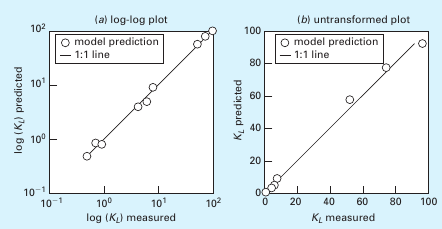
\includegraphics[width=1\linewidth]{fig_15_5}
	\caption{\textsf{Plots of predicted versus measured values of the oxygen mass-transfer coefficient as computed with multiple regression. Results are shown for (a) log transformed and (b) untransformed cases. The 1:1 line, which indicates a perfect correlation, is superimposed on both plots.}}
	\label{fig:fig_15_5}
\end{figure}

% TODO PROBLEMS 375

\label{cha:cha_P_16} %380
\chapter{Fourier Analysis}
\textbf{CHAPTER OBJECTIVES}

\noindent The primary objective of this chapter is to introduce you to Fourier analysis. The
subject, which is named after Joseph Fourier, involves identifying cycles or patterns
within a time series of data. Specific objectives and topics covered in this chapter are

\begin{itemize}
	\item Understanding sinusoids and how they can be used for curve fitting.
	\item Knowing how to use least-squares regression to fit a sinusoid to data.
	\item Knowing how to fit a Fourier series to a periodic function.
	\item Understanding the relationship between sinusoids and complex exponentials
	based on Euler's formula.
	\item Recognizing the benefits of analyzing mathematical function or signals in the frequency domain (i.e., as a function of frequency).
	\item Understanding how the Fourier integral and transform extend Fourier analysis to aperiodic functions.
	\item Understanding how the discrete Fourier transform (DFT) extends Fourier analysis
	to discrete signals.
	\item Recognizing how discrete sampling affects the ability of the DFT to distinguish
	frequencies. In particular, know how to compute and interpret the Nyquist
	frequency.
	\item Recognizing how the fast Fourier transform (FFT) provides a highly efficient
	means to compute the DFT for cases where the data record length is a power of 2.
	\item Knowing how to use the MATLAB function \texttt{fft} to compute a DFT and
	understand how to interpret the results.
	\item Knowing how to compute and interpret a power spectrum.
\end{itemize}

% TODO YOU'VE GOT A PROBLEM

AThen, predict t the beginning in the Chap. equilibrium 13, of we Chap. determined positions 8, we used the of Newton's three same system's bungee second jumpers eigenvalues law and connected force and eigenvectors
balances by cords.
to
in order to identify its resonant frequencies and principal modes of vibration. Although this analysis certainly provided useful results, it required detailed system information including
knowledge of the underlying model and parameters (i.e., the jumpers' masses and the
cords' spring constants).

So suppose that you have measurements of the jumpers' positions or velocities at discrete, equally spaced times (recall Fig. 13.1). Such information is referred to as a \textit{time series}. However, suppose further that you do not know the underlying model or the parameters needed to compute the eigenvalues. For such cases, is there any way to use the time
series to learn something fundamental about the system's dynamics?

In this chapter, we describe such an approach, \textit{Fourier analysis}, which provides a way to accomplish this objective. The approach is based on the premise that more complicated functions (e.g., a time series) can be represented by the sum of simpler trigonometric functions. As a prelude to outlining how this is done, it is useful to explore how data can be fit
with sinusoidal functions.

\label{cha:cha_P_16_1}
\section{CURVE FITTING WITH SINUSOIDAL FUNCTIONS}

\noindent A periodic function $f(t)$ is one for which

\begin{equation}
	\tag{16.1}
	f(t) = f(t + T)
\end{equation}

\noindent where T is a constant called the \textit{period} that is the smallest value of time for which Eq. (16.1) holds. Common examples include both artificial and natural signals (Fig. 16.1a).

\begin{figure}[H]
	\centering
	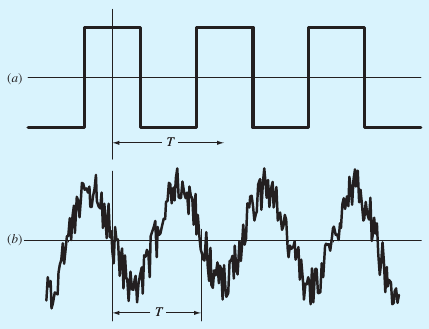
\includegraphics[width=1\linewidth]{fig_16_1}
	\caption{\textsf{Aside from trigonometric functions such as sines and cosines, periodic functions include
	idealized waveforms like the square wave depicted in (a). Beyond such artificial forms, periodic
	signals in nature can be contaminated by noise like the air temperatures shown in (b).}}
	\label{fig:fig_16_1}
\end{figure}

\begin{figure}[H]
	\centering
	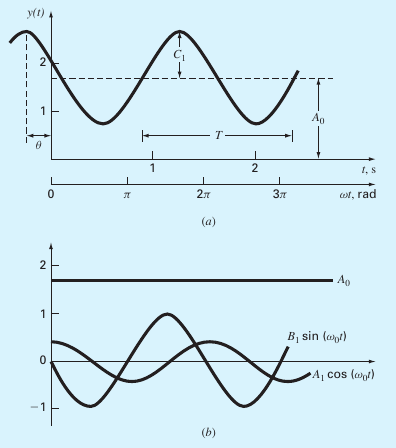
\includegraphics[width=1\linewidth]{fig_16_2}
	\caption{\textsf{(a) A plot of the sinusoidal function $y(t) = A_0 + C_1 \cos(\omega_0 t + \theta)$. For this case, $A_0 = 1.7$, $C_1 = 1$, $\omega_0 = 2 \pi / T = 2 \pi / (1.5 s)$, and $\theta = \pi / 3$ radians $= 1.0472$ ($= 0.25 s$). Other	parameters used to describe the curve are the frequency $f = \omega_0 /(2\pi)$, which or this case is 1 cycle $/ (1.5 s) = 0.6667$ Hz and the period $T = 1.5 s$. (b) An alternative expression of the same curve is $y(t) = A_0 + A_1 \cos(\omega_0 t) + B_1 \sin(\omega_0 t)$. The three components of this function are depicted in (b), where $A_1 = 0.5$ and $B_1 = -0.866$. The summation of the three curves in (b) yields the single curve in (a).}}
	\label{fig:fig_16_2}
\end{figure}

The most fundamental are sinusoidal functions. In this discussion, we will use the term \textit{sinusoid} to represent any waveform that can be described as a sine or cosine. There is no clear-cut convention for choosing either function, and in any case, the results will be identical because the two functions are simply offset in time by $\pi/2$ radians. For this chapter, we will use the cosine, which can be expressed generally as

\begin{equation}
	\tag{16.2}
	f(t) = A_0 + C_1 \cos (\omega_0 t + \theta)
\end{equation}

\noindent Inspection of Eq. (16.2) indicates that four parameters serve to uniquely characterize the
sinusoid (Fig. 16.2a):

\begin{itemize}
	\item The \textit{mean value} $A_0$ sets the average height above the abscissa.
	\item The \textit{amplitude} $C_1$ specifies the height of the oscillation.
	\item The \textit{angular frequency} $\omega_0$ characterizes how often the cycles occur.
	\item The \textit{phase angle} (or \textit{phase shift}) $\theta$ parameterizes the extent to which the sinusoid is shifted horizontally.
\end{itemize}

\begin{figure}[H]
	\centering
	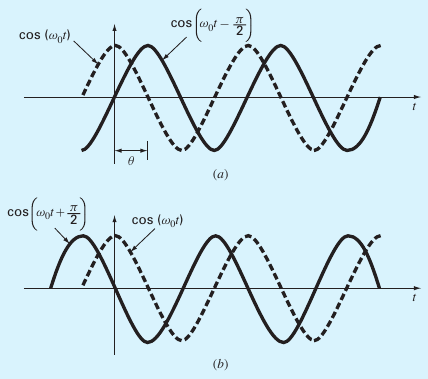
\includegraphics[width=1\linewidth]{fig_16_3}
	\caption{\textsf{Graphical depictions of (a) a lagging phase angle and (b) a leading phase angle. Note that the lagging curve in (a) can be alternatively described as $\cos(\omega_0 t + 3 \pi /2)$. In other words, if a curve lags by an angle of $\alpha$, it can also be represented as leading by $2\pi - \alpha$.}}
	\label{fig:fig_16_3}
\end{figure}

Note that the \textit{angular frequency} (in radians/time) is related to the \textit{ordinary frequency} $f$ (in cycles/time) by % TODO CITATION 383

\begin{equation}
	\tag{16.3}
	\omega_0 = 2 \pi f
\end{equation}

\noindent and the ordinary frequency in turn is related to the period $T$ by

\begin{equation}
	\tag{16.4}
	f = \frac{1}{T}
\end{equation}

In addition, the \textit{phase angle} represents the distance in radians from $t = 0$ to the point at which the cosine function begins a new cycle. As depicted in Fig. 16.3a, a negative value is referred to as a \textit{lagging phase angle} because the curve $\cos(\omega_0 t - \theta)$ begins a new cycle $\theta$ radians after $\cos(\omega_0 t)$. Thus, $\cos(\omega_0 t - \theta)$ is said to lag $\cos(\omega_0 t)$. Conversely, as in Fig. 16.3b, a positive value is referred to as a \textit{leading phase angle}.

Although Eq. (16.2) is an adequate mathematical characterization of a sinusoid, it is awkward to work with from the standpoint of curve fitting because the phase shift is included in the argument of the cosine function. This deficiency can be overcome by invoking the trigonometric identity:

\begin{equation}
	\tag{16.5}
	C_1 \cos(\omega_0 t + \theta) = C_1 [\cos(\omega_0 t + \theta) \cos(\theta) - \sin(\omega_0 t + \theta) \sin(\theta)]
\end{equation}

\noindent Substituting Eq. (16.5) into Eq. (16.2) and collecting terms gives (Fig. 16.2b)

\begin{equation}
	\tag{16.6}
	f(t) = A_0 + A_1 \cos(\omega_0 t) + B_1 \sin(\omega_0 t)
\end{equation}

\noindent where

\begin{equation}
	\tag{16.7}
	A_1 = C_1 \cos(\theta) \quad \quad B_1 = - C_1 \sin(\theta)
\end{equation}

\noindent Dividing the two parts of Eq. (16.7) gives

\begin{equation}
	\tag{16.8}
	\theta = \arctan (- \frac{B_1}{A_1})
\end{equation}

\noindent where, if $A_1 < 0$, add $\pi$ to $\theta$. Squaring and summing Eq. (16.7) leads to

\begin{equation}
	\tag{16.9}
	C_1 = \sqrt{A^2_1 + B ^2_1}
\end{equation}

\noindent Thus, Eq. (16.6) represents an alternative formulation of Eq. (16.2) that still requires four parameters but that is cast in the format of a general linear model [recall Eq. (15.7)]. As we will
discuss in the next section, it can be simply applied as the basis for a least-squares fit.

Before proceeding to the next section, however, we should stress that we could have
employed a sine rather than a cosine as our fundamental model of Eq. (16.2). For example,

\begin{equation}
	\notag
	f(t) = A_0 + C_1 \sin(\omega_0 t + \delta)
\end{equation}

\noindent could have been used. Simple relationships can be applied to convert between the two forms:

\begin{equation}
	\notag
	\sin(\omega_0 t + \delta) = \cos(\omega_0 t + \delta - \frac{\pi}{2})
\end{equation}

\noindent and

\begin{equation}
	\tag{16.10}
	\sin(\omega_0 t + \delta) = \sin(\omega_0 t + \delta + \frac{\pi}{2})
\end{equation}

\noindent In other words, $\theta = \delta - \pi/2$. The only important consideration is that one or the other format
should be used consistently. Thus, we will use the cosine version throughout our discussion.

\label{cha:cha_P_16_1_1}
\subsection{Least-Squares Fit of a Sinusoid}

\noindent Equation (16.6) can be thought of as a linear least-squares model:

\begin{equation}
	\tag{16.11}
	y = A_0 + A_1 \cos(\omega_0 t) + B_1 \sin(\omega_0 t) + e
\end{equation}

\noindent which is just another example of the general model [recall Eq. (15.7)]

\begin{equation}
	\notag
	y = a_0 z_0 + a_1 z_1 + a_2 z_2 + \cdots + a_m z_m + e
\end{equation}

\noindent where $z_0 = 1$, $z_1 = \cos(\omega_0 t)$, $z_2 = sin(\omega_0 t)$, and all other $z$'s = 0. Thus, our goal is to determine coefficient values that minimize

\begin{equation}
	\notag
	S_r = \sum ^ N _ {i=1} \{ y_i - [A_0 + A_1 \cos(\omega_0 t) + B_1 \sin(\omega_0 t)]\}^2
\end{equation}

\noindent The normal equations to accomplish this minimization can be expressed in matrix form as [recall Eq. (15.10)]

\begin{equation}
	\tag{16.12}
	\begin{bmatrix}
		N & \sum \ cos(\omega_0 t) & \sum \sin(\omega_0 t) \\
		\sum \cos(\omega_0 t) & \sum \cos^2 (\omega_0 t) & \sum \cos (\omega_0 t) \sin (\omega_0 t) \\
		\sum \sin(\omega_0 t) & \sum \cos (\omega_0 t) \sin (\omega_0 t) & \sin^2 (\omega_0 t)
	\end{bmatrix}
	\begin{Bmatrix}
		A_0 \\ B_1 \\ B_1
	\end{Bmatrix}
	=
	\begin{Bmatrix}
		\sum y \\ \sum y \cos(\omega_0 t) \\ \sum y \sin(\omega_0 t)
	\end{Bmatrix}
\end{equation}
% 385

These equations can be employed to solve for the unknown coefficients. However,
rather than do this, we can examine the special case where there are N observations equispaced at intervals of $\Delta t$ and with a total record length of $T = (N - 1)\Delta t$. For this situa-
tion, the following average values can be determined (see Prob. 16.3):

% TODO eq 16.13

\noindent Thus, for equispaced points the normal equations become

\begin{equation}
	\notag
	\begin{bmatrix}
		N & 0 & 0 \\
		0 & N/2 & 0 \\
		0 & 0 & N/2
	\end{bmatrix}
	\begin{Bmatrix}
		A_0 \\ B_1 \\ B_2
	\end{Bmatrix}
	=
	\begin{bmatrix}
		\sum y \\
		\sum y \cos(\omega_0 t) \\
		\sum y \sin(\omega_0 t)
	\end{bmatrix}
\end{equation}

\noindent The inverse of a diagonal matrix is merely another diagonal matrix whose elements are the
reciprocals of the original. Thus, the coefficients can be determined as

\begin{equation}
	\notag
	\begin{Bmatrix}
		A_0 \\ B_1 \\ B_2
	\end{Bmatrix}
	=
	\begin{bmatrix}
		1/N & 0 & 0 \\
		0 & 2/N & 0 \\
		0 & 0 & 2/N
	\end{bmatrix}
	\begin{bmatrix}
		\sum y \\
		\sum y \cos(\omega_0 t) \\
		\sum y \sin(\omega_0 t)
	\end{bmatrix}
\end{equation}

\noindent or

\begin{equation}
	\tag{16.14}
	A_0 = \frac{\sum y}{N}
\end{equation}

\begin{equation}
	\tag{16.15}
	A_1 =\frac{2}{N} \sum y \cos(\omega_0 t)
\end{equation}

\begin{equation}
	\tag{16.16}
	B_1 = \frac{2}{N} \sum y \sin(\omega_0 t)
\end{equation}

\noindent Notice that the first coefficient represents the function's average value.

% TODO example 16.1

The foregoing analysis can be extended to the general model
\begin{equation}
	\notag
	f(t) = A_0 + A_1 \cos(\omega_0 t) + B_1 \sin(\omega_0 t) + A_2 \cos(2 \omega_0 t) + B_2 \sin(2 \omega_0 t) + \cdots + A_m \cos(m \omega_0 t) + B_m \sin(m \omega_0 t)
\end{equation}

\noindent where, for equally spaced data, the coefficients can be evaluated by

\begin{equation}
	\notag
	A_0 = \frac{\sum y}{N}
\end{equation}

\begin{equation}
	\notag
	\left.
		\begin{array}{ll}
			A_j = \frac{2}{N} \sum y \cos(j \omega_0) t \\
			B_j = \frac{2}{N} \sum y \sin(j \omega_0 t)
		\end{array}
	\right \} j = 1,2, \dotsb , m
\end{equation}

%387
Although these relationships can be used to fit data in the regression sense (i.e.,$N  > 2 m + 1$), an alternative application is to employ them for interpolation or collocation - that
is, to use them for the case where the number of unknowns $2m + 1$ is equal to the number
of data points $N$. This is the approach used in the continuous Fourier series, as described
next.

\label{cha:cha_P_16_2}
\section{CONTINUOUS FOURIER SERIES}

In the course of studying heat-flow problems, Fourier showed that an arbitrary periodic
function can be represented by an infinite series of sinusoids of harmonically related
frequencies. For a function with period $T$, a continuous Fourier series can be written

\begin{equation}
	\notag
	f(t) a_0 + a_1 \cos(\omega_0 t) + b_1 \sin(\omega_0 t) +  a_2 \cos(2 \omega_0 t) + b_2 \sin(2 \omega_0 t) + \cdots
\end{equation}

\noindent or more concisely,
% TODO THIS BREAKS EVERYTHING
\begin{equation}
	\tag{16.17}
	f(t) = a_0 + \sum
\end{equation}

\noindent where the angular frequency of the first mode $(\omega_0 = 2 \pi /T)$ is called the fundamental
frequency and its constant multiples $2 \omega_0, 3 \omega_0$, etc., are called harmonics. Thus, Eq. (16.17)
expresses $f(t)$ as a linear combination of the basis functions: $1, cos( \omega_0 t), sin(\omega_0 t), cos(2 \omega_0 t),
sin(2 \omega_0 t), \dots$

The coefficients of Eq. (16.17) can be computed via

\begin{equation}
	\tag{16.18}
	a_k = \frac{2}{T} \int ^ T _ 0 f(t) \cos (k \omega_0 t) dt
\end{equation}

\noindent and

\begin{equation}
	\tag{16.19}
	b_k = \frac{2}{T} \int ^ T _ 0 f(t) \sin (k \omega_0 t) dt
\end{equation}

\noindent for $k = 1, 2, \dots$ and

\begin{equation}
	\tag{16.20}
	a_0 = \frac{1}{T} \int ^ T _ 0 f(t)dt
\end{equation}

%TODO example 16.2

Before proceeding, the Fourier series can also be expressed in a more compact form
using complex notation. This is based on \textit{Euler's formula} (Fig. 16.5):

\begin{equation}
	\tag{16.21}
	e^{\pm ix} = \cos x \pm  i \sin x
\end{equation}

\noindent where $i = \sqrt{-1}$, and $x$ is in radians. Equation (16.21) can be used to express the Fourier
series concisely as (Chapra and Canale, 2010)

\begin{equation}
	\tag{16.22}
	f(t) = \sum _ {k=-\infty} ^ {\infty} \tilde{c}_k e^{i k \omega_0 t} 
\end{equation}

\noindent where the coefficients are

\begin{equation}
	\tag{16.23}
	\tilde{c}_k = \frac{1}{T} \int ^ {T/2} _ {-T/2} f(t) e ^ {-ik \omega_0 t} dt
\end{equation}

Note that the tildes ~ are included to stress that the coefficients are complex numbers.
Because it is more concise, we will primarily use the complex form in the rest of the
chapter. Just remember, that it is identical to the sinusoidal representation.

\begin{figure}[H] % FIXME too huge
	\centering
	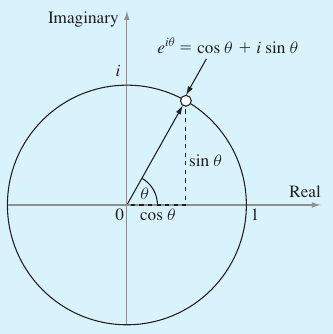
\includegraphics[width=1\linewidth]{fig_16_5}
	\caption{\textsf{Graphical depiction of Euler's formula. The rotating vector is called a phasor.}}
	\label{fig:fig_16_5}
\end{figure}

\label{cha:cha_P_16_3} %390
\section{FREQUENCY AND TIME DOMAINS}

\noindent To this point, our discussion of Fourier analysis has been limited to the \textit{time domain}. We
have done this because most of us are fairly comfortable conceptualizing a function's
behavior in this dimension. Although it is not as familiar, the \textit{frequency domain} provides an
alternative perspective for characterizing the behavior of oscillating functions.

Just as amplitude can be plotted versus time, it can also be plotted versus frequency.
Both types of expression are depicted in Fig. 16.6a, where we have drawn a threedimensional graph of a sinusoidal function:

\begin{equation}
	\notag
	f(t) = C_1 \cos(t + \frac{\pi}{2})
\end{equation} 

\begin{figure}[H] 
	\centering
	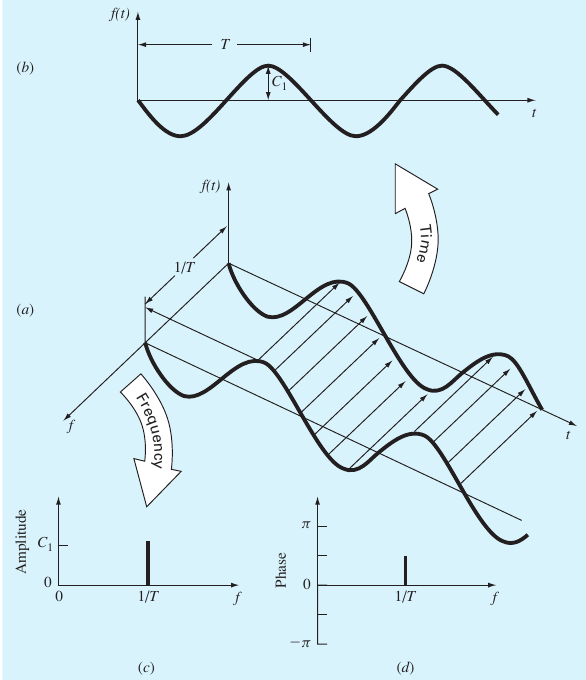
\includegraphics[width=1\linewidth]{fig_16_6}
	\caption{\textsf{(a) A depiction of how a sinusoid can be portrayed in the time and the frequency domains. The
	time projection is reproduced in (b), whereas the amplitude-frequency projection is reproduced in
	(c). The phase-frequency projection is shown in (d).}}
	\label{fig:fig_16_6}
\end{figure}

\noindent In this plot, the magnitude or amplitude of the curve $f(t)$ is the dependent variable, and time $t$
and frequency $f = \omega_0 / 2 \pi$ are the independent variables. Thus, the amplitude and the time
axes form a \textit{time plane}, and the amplitude and the frequency axes form a \textit{frequency plane}.
The sinusoid can, therefore, be conceived of as existing a distance $1/T$ out along the frequency axis and running parallel to the time axes. Consequently, when we speak about the
behavior of the sinusoid in the time domain, we mean the projection of the curve onto the
time plane (Fig. 16.6b). Similarly, the behavior in the frequency domain is merely its projection onto the frequency plane.

As in Fig. 16.6c, this projection is a measure of the sinusoid's maximum positive
amplitude $C_1$. The full peak-to-peak swing is unnecessary because of the symmetry.
Together with the location $1/T$ along the frequency axis, Fig. 16.6c now defines the
amplitude and frequency of the sinusoid. This is enough information to reproduce the
shape and size of the curve in the time domain. However, one more parameter - namely,
the phase angle - is required to position the curve relative to $t = 0$. Consequently, a
phase diagram, as shown in Fig. 16.6d, must also be included. The phase angle is determined as the distance (in radians) from zero to the point at which the positive peak
occurs. If the peak occurs after zero, it is said to be delayed (recall our discussion of lags
and leads in Sec. 16.1), and by convention, the phase angle is given a negative sign.
Conversely, a peak before zero is said to be advanced and the phase angle is positive.
Thus, for Fig. 16.6, the peak leads zero and the phase angle is plotted as $+\pi / 2$. Figure 16.7 depicts some other possibilities.

We can now see that Fig. 16.6c and $d$ provide an alternative way to present or summarize the pertinent features of the sinusoid in Fig. 16.6a. They are referred to as \textit{line spectra}.
Admittedly, for a single sinusoid they are not very interesting. However, when applied to a
more complicated situation-say, a Fourier series-their true power and value is revealed.
For example, Fig. 16.8 shows the amplitude and phase line spectra for the square-wave
function from Example 16.2.

Such spectra provide information that would not be apparent from the time domain.
This can be seen by contrasting Fig. 16.4 and Fig. 16.8. Figure 16.4 presents two alternative time domain perspectives. The first, the original square wave, tells us nothing
about the sinusoids that comprise it. The alternative is to display these sinusoids-that
is, $(4 / \pi) \cos(\omega_0 t), -(4/3 \pi) \cos(3 \omega_0 t), (4/5 \pi) \cos(5 \omega_0t ),$ etc. This alternative does
not provide an adequate visualization of the structure of these harmonics. In contrast,
Fig. 16.8a and b provide a graphic display of this structure. As such, the line spectra
represent ``fingerprints'' that can help us to characterize and understand a complicated
waveform. They are particularly valuable for nonidealized cases where they sometimes
allow us to discern structure in otherwise obscure signals. In the next section, we will
describe the Fourier transform that will allow us to extend such analyses to nonperiodic
waveforms.

\label{cha:cha_P_16_4} %391
\section{FOURIER INTEGRAL AND TRANSFORM}

\noindent Although the Fourier series is a useful tool for investigating periodic functions, there are
many waveforms that do not repeat themselves regularly. For example, a lightning bolt
occurs only once (or at least it will be a long time until it occurs again), but it will cause interference with receivers operating on a broad range of frequencies - for example, TVs,
radios, and shortwave receivers. Such evidence suggests that a nonrecurring signal such as
that produced by lightning exhibits a continuous frequency spectrum. Because such phenomena are of great interest to engineers, an alternative to the Fourier series would be valuable for analyzing these aperiodic waveforms.

\begin{figure}[H] 
	\centering
	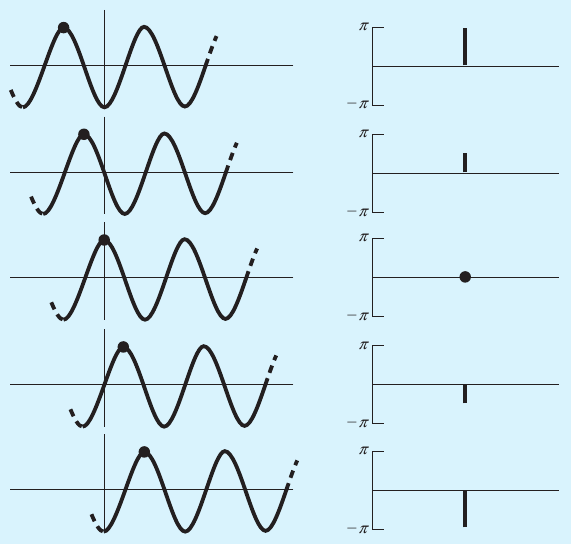
\includegraphics[width=1\linewidth]{fig_16_7}
	\caption{\textsf{Various phases of a sinusoid showing the associated phase line spectra.}}
	\label{fig:fig_16_7}
\end{figure}

The \textit{Fourier integral} is the primary tool available for this purpose. It can be derived
from the exponential form of the Fourier series [Eqs. (16.22) and (16.23)]. The transition
from a periodic to a nonperiodic function can be effected by allowing the period to approach infinity. In other words, as $T$ becomes infinite, the function never repeats itself and
thus becomes aperiodic. If this is allowed to occur, it can be demonstrated (e.g., Van
Valkenburg, 1974; Hayt and Kemmerly, 1986) that the Fourier series reduces to

\begin{equation}
	\tag{16.24}
	f(t) = \frac{1}{2 \pi} \int ^ \infty _ {-\infty} F(\omega) e ^ {i \omega t} d \omega
\end{equation}

\begin{figure}[H] 
	\centering
	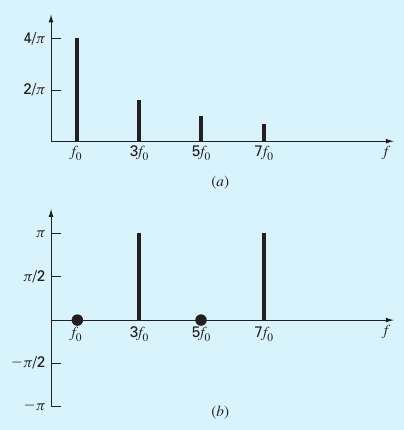
\includegraphics[width=1\linewidth]{fig_16_8}
	\caption{\textsf{(a) Amplitude and (b) phase line spectra for the square wave from Fig. 16.4.}}
	\label{fig:fig_16_8}
\end{figure}

\noindent and the coefficients become a continuous function of the frequency variable $\omega$, as in

\begin{equation}
	\tag{16.25}
	F(\omega) = \int ^ \infty _ {-\infty} f(t)e ^ {-i \omega t} dt
\end{equation}

The function $F(\omega)$, as defined by Eq. (16.25), is called the \textit{Fourier integral} of $f(t)$. In
addition, Eqs. (16.24) and (16.25) are collectively referred to as the \textit{Fourier transform}
pair. Thus, along with being called the Fourier integral, $F(\omega)$ is also called the \textit{Fourier
transform} of $f(t)$. In the same spirit, $f(t)$, as defined by Eq. (16.24), is referred to as the
\textit{inverse Fourier transform} of $F(\omega)$. Thus, the pair allows us to transform back and forth
between the time and the frequency domains for an aperiodic signal.

The distinction between the Fourier series and transform should now be quite clear.
The major difference is that each applies to a different class of functions-the series to periodic and the transform to nonperiodic waveforms. Beyond this major distinction, the two
approaches differ in how they move between the time and the frequency domains. The
Fourier series converts a continuous, periodic time-domain function to frequency-domain
magnitudes at discrete frequencies. In contrast, the Fourier transform converts a continuous time-domain function to a continuous frequency-domain function. Thus, the discrete
frequency spectrum generated by the Fourier series is analogous to a continuous frequency
spectrum generated by the Fourier transform.

Now that we have introduced a way to analyze an aperiodic signal, we will take the
final step in our development. In the next section, we will acknowledge the fact that a
signal is rarely characterized as a continuous function of the sort needed to implement
Eq. (16.25). Rather, the data are invariably in a discrete form. Thus, we will now show how
to compute a Fourier transform for such discrete measurements.

\label{cha:cha_P_16_5} %394
\section{DISCRETE FOURIER TRANSFORM (DFT)}

\noindent In engineering, functions are often represented by a finite set of discrete values. Additionally, data are often collected in or converted to such a discrete format. As depicted in
Fig. 16.9, an interval from 0 to $T$ can be divided into $n$ equispaced subintervals with widths
of $\Delta t = T /n$. The subscript $j$ is employed to designate the discrete times at which samples
are taken. Thus, $f_j$ designates a value of the continuous function $f(t)$ taken at $t_j$. Note that the
data points are specified at $j = 0, 1, 2, \dots , n - 1$. A value is not included at $j = n$. (See
Ramirez, 1985, for the rationale for excluding $f_n$.)

For the system in Fig. 16.9, a discrete Fourier transform can be written as
\begin{equation}
	\tag{16.26}
	F_k = \sum ^ {n-1} _ {j=0} f_j e ^ {-ik \omega_0 j} \quad \text{for } k=0 \text{ to } n - 1
\end{equation}

\noindent and the inverse Fourier transform as

\begin{equation}
	\tag{16.27}
	F_k = \frac{1}{n} \sum ^ {n-1} _ {k=0} F_k e ^ {ik \omega_0 j} \quad \text{for } j=0 \text{ to } n - 1
\end{equation}

\noindent where $\omega_0 = 2 \pi / n$.

\begin{figure}[H] 
	\centering
	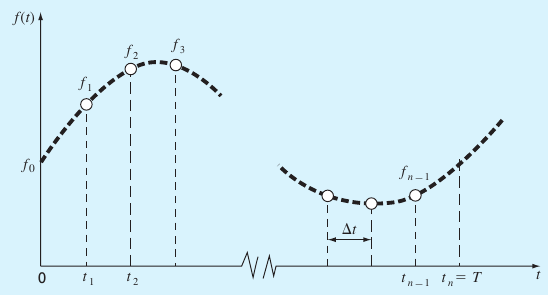
\includegraphics[width=1\linewidth]{fig_16_9}
	\caption{\textsf{The sampling points of the discrete Fourier series.}}
	\label{fig:fig_16_9}
\end{figure}

Equations (16.26) and (16.27) represent the discrete analogs of Eqs. (16.25) and
(16.24), respectively. As such, they can be employed to compute both a direct and an inverse Fourier transform for discrete data. Note that the factor $1/n$ in Eq. (16.27) is merely
a scale factor that can be included in either Eq. (16.26) or (16.27), but not both. For example, if it is shifted to Eq. (16.26), the first coefficient $F_0$ (which is the analog of the constant
$a_0$) is equal to the arithmetic mean of the samples.

Before proceeding, several other aspects of the DFT bear mentioning. The highest frequency that can be measured in a signal, called the \textit{Nyquist frequency}, is half the sampling
frequency. Periodic variations that occur more rapidly than the shortest sampled time interval cannot be detected. The lowest frequency you can detect is the inverse of the total
sample length.

As an example, suppose that you take 100 samples of data ($n = 100$ samples) at a
sample frequency of $f_s = 1000$ Hz (i.e., 1000 samples per second). This means that the
sample interval is

\begin{equation}
	\notag
	\Delta t = \frac{1}{f_s}=\frac{1}{1000 \text{ samples/s}} = 0.01 \text{ s/sample}
\end{equation}

\noindent The total sample length is 

\begin{equation}
	\notag
	t_n = \frac{n}{f_s} = \frac{100 \text{ samples}}{1000 \text{ samples/s}}=0.1 \text{ Hz}
\end{equation}

\noindent and the frequency increment is

\begin{equation}
	\notag
	\Delta f = \frac{f_s}{n} = \frac{1000 \text{ samples/s}}{100 \text{ samples}}=10 \text{ Hz}
\end{equation}

\noindent The Nyquist frequency is

\begin{equation}
	\notag
	f_{\text{max}} = 0.5 f_s = 0.5 (1000 \text{ Hz}) = 500 \text{ Hz}
\end{equation}

\noindent and the lowest detectable frequency is

\begin{equation}
	\notag
	f_{\text{min}} = \frac{1}{0.1 \text{s}} = 10 \text{ Hz}
\end{equation}

\noindent Thus, for this example, the DFT could detect signals with periods from $1/500 = 0.002 \text{s}$ up
to $1/10 = 0.1\text{s}$.

\label{cha:cha_P_16_5_1} % 395
\subsection{Fast Fourier Transform (FFT)}

\noindent Although an algorithm can be developed to compute the DFT based on Eq. (16.26), it is
computationally burdensome because $n^2$ operations are required. Consequently, for data
samples of even moderate size, the direct determination of the DFT can be extremely time
consuming.

\begin{figure}[H] 
	\centering
	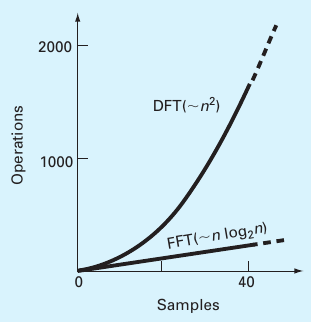
\includegraphics[width=1\linewidth]{fig_16_10}
	\caption{\textsf{Plot of number of operations vs. sample size for the standard DFT and the FFT.}}
	\label{fig:fig_16_10}
\end{figure}

The \textit{fast Fourier transform}, or \textit{FFT}, is an algorithm that has been developed to com-
pute the DFT in an extremely economical fashion. Its speed stems from the fact that it
utilizes the results of previous computations to reduce the number of operations. In particular, it exploits the periodicity and symmetry of trigonometric functions to compute
the transform with approximately $n \log_2n$ operations (Fig. 16.10). Thus, for $n = 50$ samples, the FFT is about 10 times faster than the standard DFT. For $n = 1000$, it is about
100 times faster.

The first FFT algorithm was developed by Gauss in the early nineteenth century
(Heideman et al., 1984). Other major contributions were made by Runge, Danielson,
Lanczos, and others in the early twentieth century. However, because discrete transforms
often took days to weeks to calculate by hand, they did not attract broad interest prior to the
development of the modern digital computer.

In 1965, J. W. Cooley and J. W. Tukey published a key paper in which they outlined an
algorithm for calculating the FFT. This scheme, which is similar to those of Gauss and
other earlier investigators, is called the Cooley-Tukey algorithm. Today, there are a host of
other approaches that are offshoots of this method. As described next, MATLAB offers a
function called \texttt{fft} that employs such efficient algorithms to compute the DFT.

\label{cha:cha_P_16_5_2} % 396
\subsection{MATLAB Function: \texttt{fft}}

\noindent MATLAB's \texttt{fft} function provides an efficient way to compute the DFT. A simple representation of its syntax is

\begin{lstlisting}[numbers=none]
	F = fft(f, n)
\end{lstlisting}

where \texttt{F =} a vector containing the DFT, and \texttt{f =} a vector containing the signal. The
parameter \texttt{n}, which is optional, indicates that the user wants to implement an $n$-point FFT.
If \texttt{f} has less than \texttt{n} points, it is padded with zeros and truncated if it has more.

Note that the elements in \texttt{F} are sequenced in what is called \textit{reverse-wrap-around
order}. The first half of the values are the positive frequencies (starting with the constant)
and the second half are the negative frequencies. Thus, if $n = 8$, the order is 0, 1, 2, 3, 4, -3, -2, -1. The following example illustrates the function's use to calculate the DFT of a
simple sinusoid.

%TODO example 16.3

\label{cha:cha_P_16_6}
\section{THE POWER SPECTRUM}

\noindent Beyond amplitude and phase spectra, power spectra provide another useful way to discern
the underlying harmonics of seemingly random signals. As the name implies, it derives
from the analysis of the power output of electrical systems. In terms of the DFT, a \textit{power
spectrum} consists of a plot of the power associated with each frequency component versus
frequency. The power can be computed by summing the squares of the Fourier coefficients:

\begin{equation}
	\notag
	P_k = {|\tilde{c}_k|}^2
\end{equation}

\noindent where $P_k$ is the power associated with each frequency $k \omega_0$.

% TODO example 16.4

% TODO case study 16.7

% TODO problems

\label{cha:cha_P_17} %351
\chapter{Polynomial Interpolation}
\textbf{CHAPTER OBJECTIVES}

\noindent The primary objective of this chapter is to introduce you to polynomial interpolation.
Specific objectives and topics covered are

\begin{itemize}
	\item Recognizing that evaluating polynomial coefficients with simultaneous equations is an ill-conditioned problem.
	\item  Knowing how to evaluate polynomial coefficients and interpolate with MATLAB's polyfit and polyval functions.
	\item  Knowing how to perform an interpolation with Newton's polynomial.
	\item  Knowing how to perform an interpolation with a Lagrange polynomial.
	\item  Knowing how to solve an inverse interpolation problem by recasting it as a roots problem.
	\item  Appreciating the dangers of extrapolation.
	\item  Recognizing that higher-order polynomials can manifest large oscillations.
\end{itemize}

% TODO YOU'VE GOT A PROBLEM

If we want to improve the velocity prediction for the free-falling bungee jumper, we might expand our model to account for other factors beyond mass and the drag coefficient can itself be formulated as a function of other factors such as the area of the jumper and characteristics such as the air's density and viscosity.

Air density and viscosity are commonly presented in tabular form as a function of
temperature. For example, Table 17.1 is reprinted from a popular fluid mechanics textbook
(White, 1999).

Suppose that you desired the density at a temperature not included in the table. In such
a case, you would have to interpolate. That is, you would have to estimate the value at the desired temperature based on the densities that bracket it. The simplest approach is to determine the equation for the straight line connecting the two adjacent values and use this
equation to estimate the density at the desired intermediate temperature. Although such
\textit{linear interpolation} is perfectly adequate in many cases, error can be introduced when the
data exhibit significant curvature. In this chapter, we will explore a number of different
approaches for obtaining adequate estimates for such situations.

%TODO TABLE 17.1

\label{cha:cha_P_17_1} % 406
\section{INTRODUCTION TO INTERPOLATION}

\noindent You will frequently have occasion to estimate intermediate values between precise data
points. The most common method used for this purpose is polynomial interpolation. The
general formula for an $(n - 1)$th-order polynomial can be written as

\begin{equation}
	\tag{17.1}
	f(x) = a_1 + a_2 x + a_3 x^2 + \cdots + a_n x^{n-1}
\end{equation}

For $n$ data points, there is one and only one polynomial of order $(n - 1)$ that passes through
all the points. For example, there is only one straight line (i.e., a first-order polynomial)
that connects two points (Fig. 17.1a). Similarly, only one parabola connects a set of three
points (Fig. 17.1b). \textit{Polynomial interpolation} consists of determining the unique (n - 1)th-order polynomial that fits n data points. This polynomial then provides a formula to
compute intermediate values.

Before proceeding, we should note that MATLAB represents polynomial coefficients
in a different manner than Eq. (17.1). Rather than using increasing powers of $x$, it uses decreasing powers as in

\begin{equation}
	\tag{17.2}
	f(x) = p_1 x ^ {n-1} + p_2 x ^ {n-2} + \cdots + p_{n-1} x + p_n
\end{equation}

\noindent To be consistent with MATLAB, we will adopt this scheme in the following section.

\begin{figure}[H] 
	\centering
	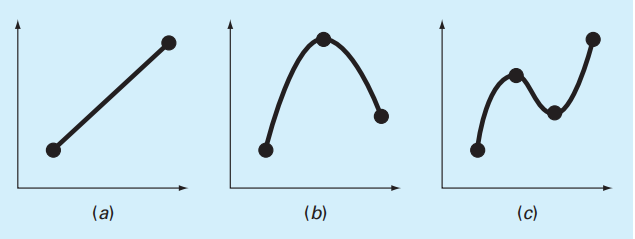
\includegraphics[width=1\linewidth]{fig_17_1}
	\caption{\textsf{Examples of interpolating polynomials: (a) first-order (linear) connecting two points,
	(b) second-order (quadratic or parabolic) connecting three points, and (c) third-order (cubic)
	connecting four points.}}
	\label{fig:fig_17_1}
\end{figure}

\label{cha:cha_P_17_1_1}
\subsection{Determining Polynomial Coefficients}

\noindent A straightforward way for computing the coefficients of Eq. (17.2) is based on the fact that
$n$ data points are required to determine the n coefficients. As in the following example, this
allows us to generate n linear algebraic equations that we can solve simultaneously for the
coefficients.

% TODO example 17.1

Although the approach in Example 17.1 provides an easy way to perform interpola-
tion, it has a serious deficiency. To understand this flaw, notice that the coefficient matrix
in Example 17.1 has a decided structure. This can be seen clearly by expressing it in general terms:

\begin{equation}
	\tag{17.3}
	\begin{bmatrix}
		x ^ 2 _ 1 & x_1 & 1 \\
		x ^ 2 _ 2 & x_2 & 1 \\
		x ^ 2 _ 3 & x_3 & 1
	\end{bmatrix}
	\begin{Bmatrix}
		p_1 \\ p_2 \\ p_3
	\end{Bmatrix}
	=
	\begin{Bmatrix}
		f(x_1) \\
		f(x_2) \\
		f(x_3)
	\end{Bmatrix}
\end{equation}

Coefficient matrices of this form are referred to as \textit{Vandermonde matrices}. Such matrices are very ill-conditioned. That is, their solutions are very sensitive to round-off errors.
This can be illustrated by using MATLAB to compute the condition number for the coefficient matrix from Example 17.1 as

\begin{lstlisting}[numbers=none]
	>> cond(A)
ans =
	5.8932e+006
\end{lstlisting}

This condition number, which is quite large for a $3 \times 3$ matrix, implies that about six digits
of the solution would be questionable. The ill-conditioning becomes even worse as the
number of simultaneous equations becomes larger.

As a consequence, there are alternative approaches that do not manifest this shortcoming. In this chapter, we will also describe two alternatives that are well-suited for
computer implementation: the Newton and the Lagrange polynomials. Before doing this,
however, we will first briefly review how the coefficients of the interpolating polynomial
can be estimated directly with MATLAB's built-in functions.

\label{cha:cha_P_17_1_2}
\subsection{MATLAB Functions: \texttt{polyfit} and \texttt{polyval}}

\noindent Recall from Section 14.5.2, that the \texttt{polyfit} function can be used to perform polynomial
regression. In such applications, the number of data points is greater than the number of
coefficients being estimated. Consequently, the least-squares fit line does not necessarily
pass through any of the points, but rather follows the general trend of the data.

For the case where the number of data points equals the number of coefficients, \texttt{polyfit} performs interpolation. That is, it returns the coefficients of the polynomial that pass
directly through the data points. For example, it can be used to determine the coefficients
of the parabola that passes through the last three density values from Table 17.1:

\begin{lstlisting}[numbers=none]
>> format long
>> T = [300 400 500];
>> density = [0.616 0.525 0.457];
>> p = polyfit(T,density,2)
p =
	0.00000115000000
	-0.00171500000000
	1.02700000000000
\end{lstlisting}

\noindent We can then use the \texttt{polyval} function to perform an interpolation as in

\begin{lstlisting}[numbers=none]
>> d = polyval(p,350)
d =
	0.56762500000000
\end{lstlisting}

\noindent These results agree with those obtained previously in Example 17.1 with simultaneous equations.

\label{cha:cha_P_17_2}
\section{NEWTON INTERPOLATING POLYNOMIAL}

\noindent There are a variety of alternative forms for expressing an interpolating polynomial beyond
the familiar format of Eq. (17.2). Newton's interpolating polynomial is among the most
popular and useful forms. Before presenting the general equation, we will introduce the
first- and second-order versions because of their simple visual interpretation.

\label{cha:cha_P_17_2_1}
\subsection{Linear Interpolation}

\noindent The simplest form of interpolation is to connect two data points with a straight line. This
technique, called \textit{linear interpolation}, is depicted graphically in Fig. 17.2. Using similar
triangles,

\begin{equation}
	\tag{17.4}
	\frac{f_1(x)-f(x_1)}{x - x_1} = \frac{f(x_2) - f(x_1)}{x_2 - x_1}
\end{equation}

\noindent which can be rearranged to yield

\begin{equation}
	\tag{17.5}
	f_1(x) = f(x_1) + \frac{f(x_2) - f(x_1)}{x_2 - x_1} (x - x_1)
\end{equation}

\noindent which is the \textit{Newton linear-interpolation formula}. The notation $f_1 (x)$ designates that this
is a first-order interpolating polynomial. Notice that besides representing the slope of the
line connecting the points, the term $[f(x_2) - f(x_1)]/(x_2 - x_1)$ is a finite-difference approximation of the first derivative [recall Eq. (4.20)]. In general, the smaller the interval
between the data points, the better the approximation. This is due to the fact that, as the
interval decreases, a continuous function will be better approximated by a straight line.
This characteristic is demonstrated in the following example.

\begin{figure}[H] 
	\centering
	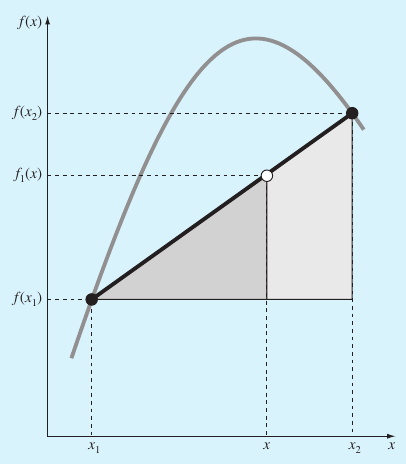
\includegraphics[width=1\linewidth]{fig_17_2}
	\caption{\textsf{Graphical depiction of linear interpolation. The shaded areas indicate the similar triangles used
	to derive the Newton linear-interpolation formula [Eq. (17.5)].}}
	\label{fig:fig_17_2}
\end{figure}

% TODO example 17.2

\label{cha:cha_P_17_2_2}
\subsection{Quadratic Interpolation}

\noindent The error in Example 17.2 resulted from approximating a curve with a straight line. Consequently, a strategy for improving the estimate is to introduce some curvature into the line
connecting the points. If three data points are available, this can be accomplished with a
second-order polynomial (also called a quadratic polynomial or a parabola). A particularly
convenient form for this purpose is

\begin{equation}
	\tag{17.6}
	f_2(x) = b_1 + b_2 (x - x_1) + b_3 (x-x_1) (x - x_2)
\end{equation}

A simple procedure can be used to determine the values of the coefficients. For $b_1$,
Eq. (17.6) with $x = x_1$ can be used to compute

\begin{equation}
	\tag{17.7}
	b_1 = f(x_1)
\end{equation}

\noindent Equation (17.7) can be substituted into Eq. (17.6), which can be evaluated at $x = x_2$ for

\begin{equation}
	\tag{17.8}
	b_2 = \frac{f(x_2) - f(x_1)}{x_2 - x_1}
\end{equation}

\noindent Finally, Eqs. (17.7) and (17.8) can be substituted into Eq. (17.6), which can be evaluated at
$x = x_3$ and solved (after some algebraic manipulations) for

\begin{equation}
	\tag{17.9}
	b_3 = \frac{
		\frac{f(x_3) - f(x_2)}{x_3 - x_2} - \frac{f(x_2) - f(x_1)}{x_2 - x_1}
	}{x_3 - x_1}
\end{equation}

Notice that, as was the case with linear interpolation, $b_2$ still represents the slope of the
line connecting points $x_1$ and $x_2$. Thus, the first two terms of Eq. (17.6) are equivalent to
linear interpolation between $x_1$ and $x_2$, as specified previously in Eq. (17.5). The last term,
$b_3 (x - x_1 )(x - x_2)$, introduces the second-order curvature into the formula.

Before illustrating how to use Eq. (17.6), we should examine the form of the coefficient $b_3$. It is very similar to the finite-difference approximation of the second derivative
introduced previously in Eq. (4.27). Thus, Eq. (17.6) is beginning to manifest a structure
that is very similar to the Taylor series expansion. That is, terms are added sequentially to
capture increasingly higher-order curvature.

% TODO example 17.3

\label{cha:cha_P_17_2_3} % 413
\subsection{General Form of Newton's Interpolating Polynomials}

\noindent The preceding analysis can be generalized to fit an $(n - 1)$th-order polynomial to $n$ data
points. The $(n - 1)$th-order polynomial is

\begin{equation}
	\tag{17.10}
	f_{n-1}(x) = b_1 + b_2 (x - x_1) + \cdots + b_n (x - x_1) (x - x_2) \cdots (x - x_{n-1})
\end{equation}

\noindent As was done previously with linear and quadratic interpolation, data points can be used to
evaluate the coefficients $b_1 , b_2 , \dots , b_n$. For an $(n - 1)$th-order polynomial, $n$ data points
are required: $[x_1 , f (x_1)], [x_2 , f (x_2)], \dots , [x_n , f (x_n )]$. We use these data points and the
following equations to evaluate the coefficients:

\begin{equation}
	\tag{17.11}
	b_1 = f(x_1)
\end{equation}

\begin{equation}
	\tag{17.12}
	b_2 = f[x_2,x_1]
\end{equation}

\begin{equation}
	\tag{17.13}
	b_3 = f[x_3, x_2, x_1]
\end{equation}

\begin{equation}
	\notag
	\vdots 
\end{equation}

\begin{equation}
	\tag{17.14}
	b_n = f[x_n, x_{n-1}, \dots, x_1]
\end{equation}

\noindent where the bracketed function evaluations are finite divided differences. For example, the
first finite divided difference is represented generally as

\begin{equation}
	\tag{17.15}
	f[x_i, x_j] = \frac{f(x_i) - f(x_j)}{x_i - x_j}
\end{equation}

\noindent The second finite divided difference, which represents the difference of two first divided
differences, is expressed generally as

\begin{equation}
	\tag{17.16}
	f[x_i, x_j, x_k] = \frac{f[x_i, x_j] - f[x_j, x_k]}{x_i - x_k}
\end{equation}

\noindent Similarly, the $n$th finite divided difference is

\begin{equation}
	\tag{17.17}
	f[x_n,x_{n-1}, \dots, x_2, x_1] = \frac{f[x_n,x_{n-1}, \dots, x_2]- f[x_{n-1}, \dots, x_2, x_1]}{x_n - x_1}
\end{equation}

\begin{figure}[H] 
	\centering
	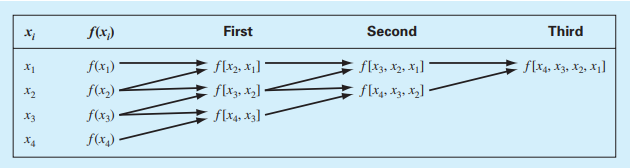
\includegraphics[width=1\linewidth]{fig_17_5}
	\caption{\textsf{Graphical depiction of the recursive nature of finite divided differences. This representation is
	referred to as a divided difference table.}}
	\label{fig:fig_17_5}
\end{figure}

\noindent These differences can be used to evaluate the coefficients in Eqs. (17.11) through (17.14),
which can then be substituted into Eq. (17.10) to yield the general form of Newton's inter-
polating polynomial:

\begin{equation}
	\tag{17.18}
	f_{n-1} (x) = f(x_1) + (x - x_1) f[x_2, x_1] + (x - x_1) (x - x_2) f[x_3,x_2,x_1] + \cdots + (x - x_1) (x - x_2) \cdots (x - x_{n-1}) f[x_n, x_{n-1}, \dots,x_2,x_1]
\end{equation}

We should note that it is not necessary that the data points used in Eq. (17.18) be
equally spaced or that the abscissa values necessarily be in ascending order, as illustrated
in the following example. However, the points should be ordered so that they are centered
around and as close as possible to the unknown. Also, notice how Eqs. (17.15) through
(17.17) are recursive-that is, higher-order differences are computed by taking differences
of lower-order differences (Fig. 17.5). This property will be exploited when we develop an
efficient M-file to implement the method.

% TODO example 17.4

\label{cha:cha_P_17_2_4} % 416
\subsection{MATLAB M-file: \texttt{Newtint}}

\noindent It is straightforward to develop an M-file to implement Newton interpolation. As in Fig. 17.7,
the first step is to compute the finite divided differences and store them in an array. The differences are then used in conjunction with Eq. (17.18) to perform the interpolation.

An example of a session using the function would be to duplicate the calculation we
just performed in Example 17.3:

\begin{lstlisting}[numbers=none]
>> format long
>> x = [1 4 6 5]';
>> y = log(x);
>> Newtint(x,y,2)
ans =
	0.62876857890841
\end{lstlisting}

\begin{figure}[H] 
	\centering
	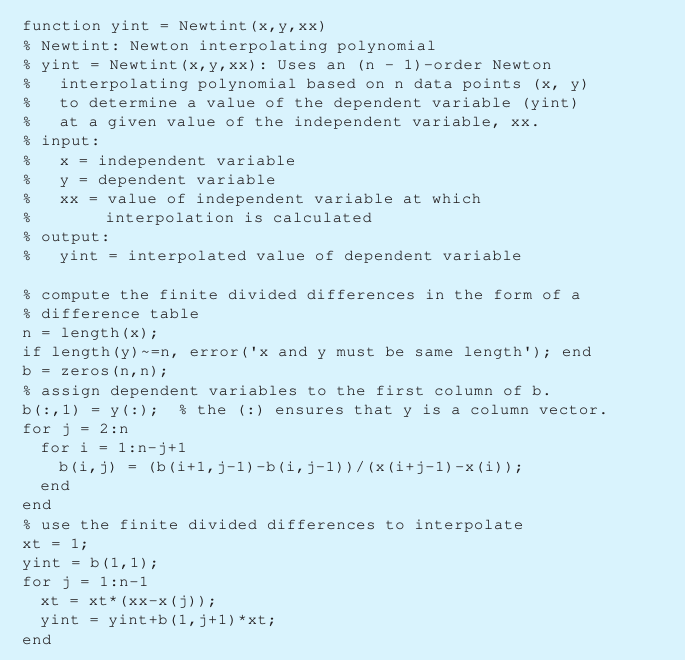
\includegraphics[width=1\linewidth]{fig_17_7}
	\caption{\textsf{An M-file to implement Newton interpolation.}}
	\label{fig:fig_17_7}
\end{figure}

\label{cha:cha_P_17_3}
\section{LAGRANGE INTERPOLATING POLYNOMIAL}

\noindent Suppose we formulate a linear interpolating polynomial as the weighted average of the two
values that we are connecting by a straight line:

\begin{equation}
	\tag{17.19}
	f(x) = L_1 f(x_1) L_2 f(x_2)
\end{equation}

\noindent where the $L$'s are the weighting coefficients. It is logical that the first weighting coefficient
is the straight line that is equal to 1 at $x_1$ and 0 at $x_2$:

\begin{equation}
	\notag
	L_1 = \frac{x - x_2}{x_1 - x_2}
\end{equation}

\noindent Similarly, the second coefficient is the straight line that is equal to 1 at $x_2$ and 0 at $x_1$:

\begin{equation}
	\notag
	L_2 = \frac{x - x_1}{x_2 - x_1}
\end{equation}

\noindent Substituting these coefficients into Eq. 17.19 yields the straight line that connects the
points (Fig. 17.8):

\begin{equation}
	\tag{17.20}
	f_1(x) = \frac{x - x_2}{x_1 - x_2} f(x_1) + \frac{x - x_1}{x_2 - x_1} f(x_2)
\end{equation}

\noindent where the nomenclature $f_1(x)$ designates that this is a first-order polynomial. Equation (17.20) is referred to as the \textit{linear Lagrange interpolating polynomial}.

The same strategy can be employed to fit a parabola through three points. For this case
three parabolas would be used with each one passing through one of the points and equaling zero at the other two. Their sum would then represent the unique parabola that connects
the three points. Such a second-order Lagrange interpolating polynomial can be written as

\begin{equation}
	\tag{17.21}
	f_2(x) = \frac{(x - x_2) (x - x_3)}{(x_1 - x_2)(x_1 - x_3)} f(x_1) + \frac{(x - x_1) (x - x_3)}{(x_2 - x_1) (x_2 - x_3)} f(x_2) + \frac{(x - x_1) (x - x_2)}{(x_3 - x_1) (x_3 - x_2)} f(x_3)
\end{equation}

\noindent Notice how the first term is equal to $f (x_1 )$ at $x_1$ and is equal to zero at $x_2$ and $x_3$ . The other
terms work in a similar fashion.

Both the first- and second-order versions as well as higher-order Lagrange polynomials can be represented concisely as

\begin{equation}
	\tag{17.22}
	f_{n-1}(x) = \sum ^ n _ {i=1} L_i (x) f(x_i)
\end{equation}

\noindent where

\begin{equation}
	\tag{17.23}
	L_i (x) = \prod ^n _{j=1, j \neq i} \frac{x - x_j}{x_i - x_j}
\end{equation}

\noindent where $n$ = the number of data points and $\prod$ designates the ``product of.''

\begin{figure}[H] 
	\centering
	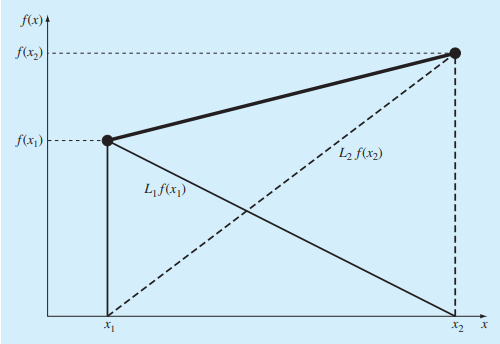
\includegraphics[width=1\linewidth]{fig_17_8}
	\caption{\textsf{A visual depiction of the rationale behind Lagrange interpolating polynomials. The figure shows
	the first-order case. Each of the two terms of Eq. (17.20) passes through one of the points and
	is zero at the other. The summation of the two terms must, therefore, be the unique straight line
	that connects the two points.}}
	\label{fig:fig_17_8}
\end{figure}

% TODO example 17.5

\label{cha:cha_P_17_3_1} % 419
\subsection{MATLAB M-file: \texttt{Lagrange}}

\noindent It is straightforward to develop an M-file based on Eqs. (17.22) and (17.23). As in
Fig. 17.9, the function is passed two vectors containing the independent (\texttt{x}) and the
dependent (\texttt{y}) variables. It is also passed the value of the independent variable where you
want to interpolate (\texttt{xx}). The order of the polynomial is based on the length of the \texttt{x} vector
that is passed. If \texttt{n} values are passed, an $(n - 1)$th order polynomial is fit.

\begin{figure}[H] 
	\centering
	\begin{lstlisting}[numbers=none]
function yint = Lagrange(x,y,xx)
% Lagrange: Lagrange interpolating polynomial
% 	yint = Lagrange(x,y,xx): Uses an (n - 1)-order
% 		Lagrange interpolating polynomial based on n data points
% 		to determine a value of the dependent variable (yint) at
% 		a given value of the independent variable, xx.
% input:
% 	x = independent variable
% 	y = dependent variable
% 	xx = value of independent variable at which the
% 		interpolation is calculated
% output:
% 		yint = interpolated value of dependent variable

n = length(x);
if length(y)~=n, error('x and y must be same length'); end
s = 0;
for i = 1:n
	product = y(i);
	for j = 1:n
		if i ~= j
			product = product*(xx-x(j))/(x(i)-x(j));
		end
	end
	s = s+product;
end
yint = s;
	\end{lstlisting}
	\caption{\textsf{An M-file to implement Lagrange interpolation.}}
	\label{fig:fig_17_9}
\end{figure}

An example of a session using the function would be to predict the density of air at
1 atm pressure at a temperature of $15^\circ$C: based on the first four values from Table 17.1.
Because four values are passed to the function, a third-order polynomial would be implemented by the \texttt{Lagrange} function to give:

\begin{lstlisting}[numbers=none]
>> format long
>> T = [-40 0 20 50];
>> d = [1.52 1.29 1.2 1.09];
>> density = Lagrange(T,d,15)

density =
	1.22112847222222
\end{lstlisting}

\label{cha:cha_P_17_4} % 420
\section{INVERSE INTERPOLATION}

\noindent As the nomenclature implies, the $f (x)$ and $x$ values in most interpolation contexts are the
dependent and independent variables, respectively. As a consequence, the values of the $x$'s
are typically uniformly spaced. A simple example is a table of values derived for the function
$f (x) = 1/x$:

% TODO table?

Now suppose that you must use the same data, but you are given a value for $f (x)$ and
must determine the corresponding value of $x$. For instance, for the data above, suppose that
you were asked to determine the value of $x$ that corresponded to $f (x) = 0.3$. For this case,
because the function is available and easy to manipulate, the correct answer can be determined directly as $x = 1/0.3 = 3.3333$.

Such a problem is called inverse interpolation. For a more complicated case, you
might be tempted to switch the $f (x)$ and $x$ values [i.e., merely plot $x$ versus $f (x)$] and use
an approach like Newton or Lagrange interpolation to determine the result. Unfortunately,
when you reverse the variables, there is no guarantee that the values along the new abscissa
[the $f (x)$'s] will be evenly spaced. In fact, in many cases, the values will be ``telescoped.''
That is, they will have the appearance of a logarithmic scale with some adjacent points
bunched together and others spread out widely. For example, for $f (x) = 1/x$ the result is

% TODO table

Such nonuniform spacing on the abscissa often leads to oscillations in the resulting interpolating polynomial. This can occur even for lower-order polynomials. An alternative
strategy is to fit an nth-order interpolating polynomial, $f_n (x)$, to the original data [i.e., with
$f (x)$ versus $x$]. In most cases, because the $x$'s are evenly spaced, this polynomial will not
be ill-conditioned. The answer to your problem then amounts to finding the value of $x$ that
makes this polynomial equal to the given $f (x)$. Thus, the interpolation problem reduces to
a roots problem!

For example, for the problem just outlined, a simple approach would be to fit a quadratic polynomial to the three points: $(2, 0.5)$, $(3, 0.3333)$, and $(4, 0.25)$. The result would be

\begin{equation}
	\notag
	f_2 (x) =  0.041667x^2 - 0.375x + 1.08333
\end{equation}

\noindent The answer to the inverse interpolation problem of finding the $x$ corresponding to
$f (x) = 0.3$ would therefore involve determining the root of

\begin{equation}
	\notag
	0.3 = 0.041667x^2 - 0.375x + 1.08333
\end{equation}

\noindent For this simple case, the quadratic formula can be used to calculate

\begin{equation}
	\notag
	x = \frac{0.375 \pm \sqrt{(-0.375)^2 - 4(0.041667)0.78333}}{2(0.041667)} = 
	\begin{matrix}
		5.704158 \\ 3.295842
	\end{matrix}
\end{equation}

\noindent Thus, the second root, $3.296$, is a good approximation of the true value of $3.333$. If additional accuracy were desired, a third- or fourth-order polynomial along with one of the
root-location methods from Chaps. 5 or 6 could be employed.

\label{cha:cha_P_17_5} % 421
\section{EXTRAPOLATION AND OSCILLATIONS}

\noindent Before leaving this chapter, there are two issues related to polynomial interpolation that
must be addressed. These are extrapolation and oscillations.

\label{cha:cha_P_17_5_1} 
\subsection{Extrapolation}

\noindent Extrapolation is the process of estimating a value of $f (x)$ that lies outside the range of the
known base points, $x_1 , x_2, \dots , x_n$. As depicted in Fig. 17.10, the open-ended nature of extrapolation represents a step into the unknown because the process extends the curve
beyond the known region. As such, the true curve could easily diverge from the prediction.
Extreme care should, therefore, be exercised whenever a case arises where one must
extrapolate.

\begin{figure}[H] 
	\centering
	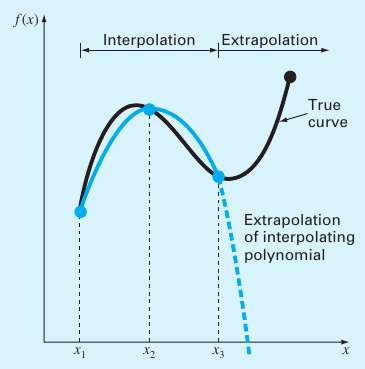
\includegraphics[width=1\linewidth]{fig_17_10}
	\caption{\textsf{Illustration of the possible divergence of an extrapolated prediction. The extrapolation is based
	on fitting a parabola through the first three known points.}}
	\label{fig:fig_17_10}
\end{figure}

% TODO example 17.6

\label{cha:cha_P_17_5_2} 
\subsection{Extrapolation}

\noindent Although ``more is better'' in many contexts, it is absolutely not true for polynomial interpolation. Higher-order polynomials tend to be very ill-conditioned - that is, they tend to be
highly sensitive to round-off error. The following example illustrates this point nicely.

% TODO example 17.7

% TODO problems

\end{document}
% TODO figure references, examples, align left math expressions